\documentclass{article}

% --- Korean translation support (xelatex + kotex) ---
\usepackage{kotex}
\usepackage{fontspec}
\setmainfont{NanumMyeongjo}[AutoFakeSlant=0.167]
\setsansfont{NanumGothic}[AutoFakeSlant=0.167]
\setmainhangulfont{NanumMyeongjo}[AutoFakeSlant=0.167]
\setsanshangulfont{NanumGothic}[AutoFakeSlant=0.167]
\setmonohangulfont{NanumGothicCoding}[AutoFakeSlant=0.167]
\setmonofont{NanumGothicCoding}[AutoFakeSlant=0.167]
\linespread{1.21}\selectfont
\renewcommand{\figurename}{그림}
\renewcommand{\tablename}{표}
\setlength{\parindent}{1.2em}
% --- end Korean support ---


% if you need to pass options to natbib, use, e.g.:
\PassOptionsToPackage{numbers, compress}{natbib}
% before loading neurips_2026

% The authors should use one of these tracks.
% Before accepting by the NeurIPS conference, select one of the options below.
% 0. "default" for submission
\usepackage[main,final]{neurips_2026}
% the "default" option is equal to the "main" option, which is used for the Main Track with double-blind reviewing.
% 1. "main" option is used for the Main Track
%  \usepackage[main]{neurips_2026}
% 2. "position" option is used for the Position Paper Track
%  \usepackage[position]{neurips_2026}
% 3. "eandd" option is used for the Evaluations & Datasets Track
 % \usepackage[eandd]{neurips_2026}
 % if you need to opt-in for a single-blind submission in the E&D track:
 %\usepackage[eandd, nonanonymous]{neurips_2026}
% 4. "creativeai" option is used for the Creative AI Track
%  \usepackage[creativeai]{neurips_2026}
% 5. "sglblindworkshop" option is used for the Workshop with single-blind reviewing
 % \usepackage[sglblindworkshop]{neurips_2026}
% 6. "dblblindworkshop" option is used for the Workshop with double-blind reviewing
%  \usepackage[dblblindworkshop]{neurips_2026}

% After being accepted, the authors should add "final" behind the track to compile a camera-ready version.
% 1. Main Track
 % \usepackage[main, final]{neurips_2026}
% 2. Position Paper Track
%  \usepackage[position, final]{neurips_2026}
% 3. Evaluations & Datasets Track
 % \usepackage[eandd, final]{neurips_2026}
% 4. Creative AI Track
%  \usepackage[creativeai, final]{neurips_2026}
% 5. Workshop with single-blind reviewing
%  \usepackage[sglblindworkshop, final]{neurips_2026}
% 6. Workshop with double-blind reviewing
%  \usepackage[dblblindworkshop, final]{neurips_2026}
% Note. For the workshop paper template, both \title{} and \workshoptitle{} are required, with the former indicating the paper title shown in the title and the latter indicating the workshop title displayed in the footnote.
% For workshops (5., 6.), the authors should add the name of the workshop, "\workshoptitle" command is used to set the workshop title.
% \workshoptitle{WORKSHOP TITLE}

% "preprint" option is used for arXiv or other preprint submissions
 % \usepackage[preprint]{neurips_2026}

% to avoid loading the natbib package, add option nonatbib:
%    \usepackage[nonatbib]{neurips_2026}

\usepackage{float}          % table float utilities
\usepackage{placeins}       % keep floats before later sections
\usepackage{hyperref}       % hyperlinks
\usepackage{url}            % simple URL typesetting
\usepackage{booktabs}       % professional-quality tables
\usepackage{amsfonts}       % blackboard math symbols
\usepackage{nicefrac}       % compact symbols for 1/2, etc.
\usepackage{microtype}      % microtypography
\usepackage[table]{xcolor}  % colors
\usepackage{multirow}       % multirow table cells
\usepackage{anyfontsize}    % support arbitrary font sizes
\usepackage{weibo_report}   % Weibo technical report style

\definecolor{vibebg}{HTML}{FFF0F0}
\definecolor{vibered}{HTML}{D7192A}
\newcommand{\na}{--}
\newcommand{\our}[1]{\textbf{#1}}
\newcommand{\clrscore}[1]{\textbf{\textcolor{vibered}{#1}}}

\renewcommand{\topfraction}{0.95}
\renewcommand{\textfraction}{0.05}
\renewcommand{\floatpagefraction}{0.85}

\weibologo{logo.pdf}
\weiboheader{VibeThinker 3B 기술 보고서}
\title{VibeThinker-3B: 소형 언어 모델에서 검증 가능한 추론의 프런티어 탐색}


% ===== Weibo Author Setup =====
% Format: bold names with superscript affiliations, then numbered affiliations below
\weiboauthors{%
  % \textbf{Sen Xu},\enspace
  % \textbf{Sen Xu},\enspace
  % \textbf{Sen Xu},\enspace
  % \textbf{Sen Xu},\enspace
  % \textbf{Sen Xu},\enspace
  % \textbf{Authors},\enspace
  % \textbf{Authors},\enspace
Sen Xu,\enspace
  Shixi Liu,\enspace
  Wei Wang,\enspace
  Jixin Min,\enspace
  Yingwei Dai,\enspace
  Zhibin Yin,\enspace \\
  Yirong Chen,\enspace
  Xin Zhou,\enspace
  Junlin Zhang \enspace
  % \textbf{Alice M.~Neuron}$^{2}$,\enspace
  % \textbf{Charlie R.~Dendrite}$^{*,1,2,\dagger}$%
}

\weiboaffils{%
  % $^1$Weibo, \quad $^2$Cranberry-Lemon University%
Sina Weibo Inc.
}

% \weibonotes{%
%   $^*$Correspondence: \{xusen1,junlin6\} \texttt{@staff.weibo.com}%
% }

\weibodate{2026년 6월 15일}
\weibogithub{\texttt{https://github.com/WeiboAI/VibeThinker}}
\weibohuggingface{\texttt{https://huggingface.co/WeiboAI/VibeThinker-3B}}
\weibocorrespondence{\{xusen1,\,junlin6\} \texttt{@staff.weibo.com}}


\begin{document}

\maketitle
\enlargethispage{3\baselineskip}


\begin{abstract}
이 기술 보고서는 엄격한 소규모 모델 체제 내에서 검증 가능한 추론이 얼마나 멀리 추진될 수 있는지 조사하기 위해 개발된 3B 매개변수를 갖춘 컴팩트한 밀도 모델인 VibeThinker-3B를 소개합니다. Spectrum-to-Signal 사후 훈련 패러다임을 기반으로 커리큘럼 기반 감독 미세 조정, 다중 도메인 강화 학습 및 오프라인 자체 증류를 포함하는 최적화된 파이프라인을 통해 모델을 체계적으로 향상합니다. 실험적 평가는 VibeThinker-3B가 매우 까다롭고 검증 가능한 작업에서 최전선 수준의 성능을 달성한다는 것을 보여줍니다. 구체적으로 AIME26에서 94.3점(클레임 수준 테스트 시간 조정을 통해 97.1로 향상), LiveCodeBench v6에서 80.2 Pass@1을 획득했으며 최근 보이지 않는 LeetCode 콘테스트에서 96.1\% 승인률로 강력한 배포 외 일반화를 보여줍니다. 이는 DeepSeek V3.2, GLM-5 및 Gemini 3 Pro와 같이 훨씬 더 큰 주력 모델과 일치하거나 초과하는 1차 추론 시스템의 성능 대역에 효과적으로 배치됩니다. 또한 IFEval에서 93.4점은 이러한 극단적인 추론 향상이 엄격한 명령어 제어 가능성을 손상시키지 않는다는 것을 확인시켜 줍니다. 이전 1.5B 작업을 확장한 이러한 발견은 검증 가능한 추론을 컴팩트 추론 코어로 압축할 수 있는 것으로 보는 파라메트릭 압축 범위 가설에 동기를 부여하는 반면, 개방형 지식과 범용 역량은 사실, 개념 및 롱테일 시나리오에 대한 광범위한 매개변수 적용 범위를 요구합니다. 이러한 관점은 콤팩트 모델이 단순히 배포 효율성이 뛰어난 대체 제품이 아니라 매개변수 밀도가 높은 역량 체제에서 최전선 수준의 성능을 향한 보완적인 경로임을 시사합니다.
\end{abstract}

\begin{figure}[H]
\centering
    % Alternative: original v3 with standard legend.
    % \includegraphics[width=\textwidth]{image/v3_clr_soft_brand_reasoning_hero_vector.pdf}
    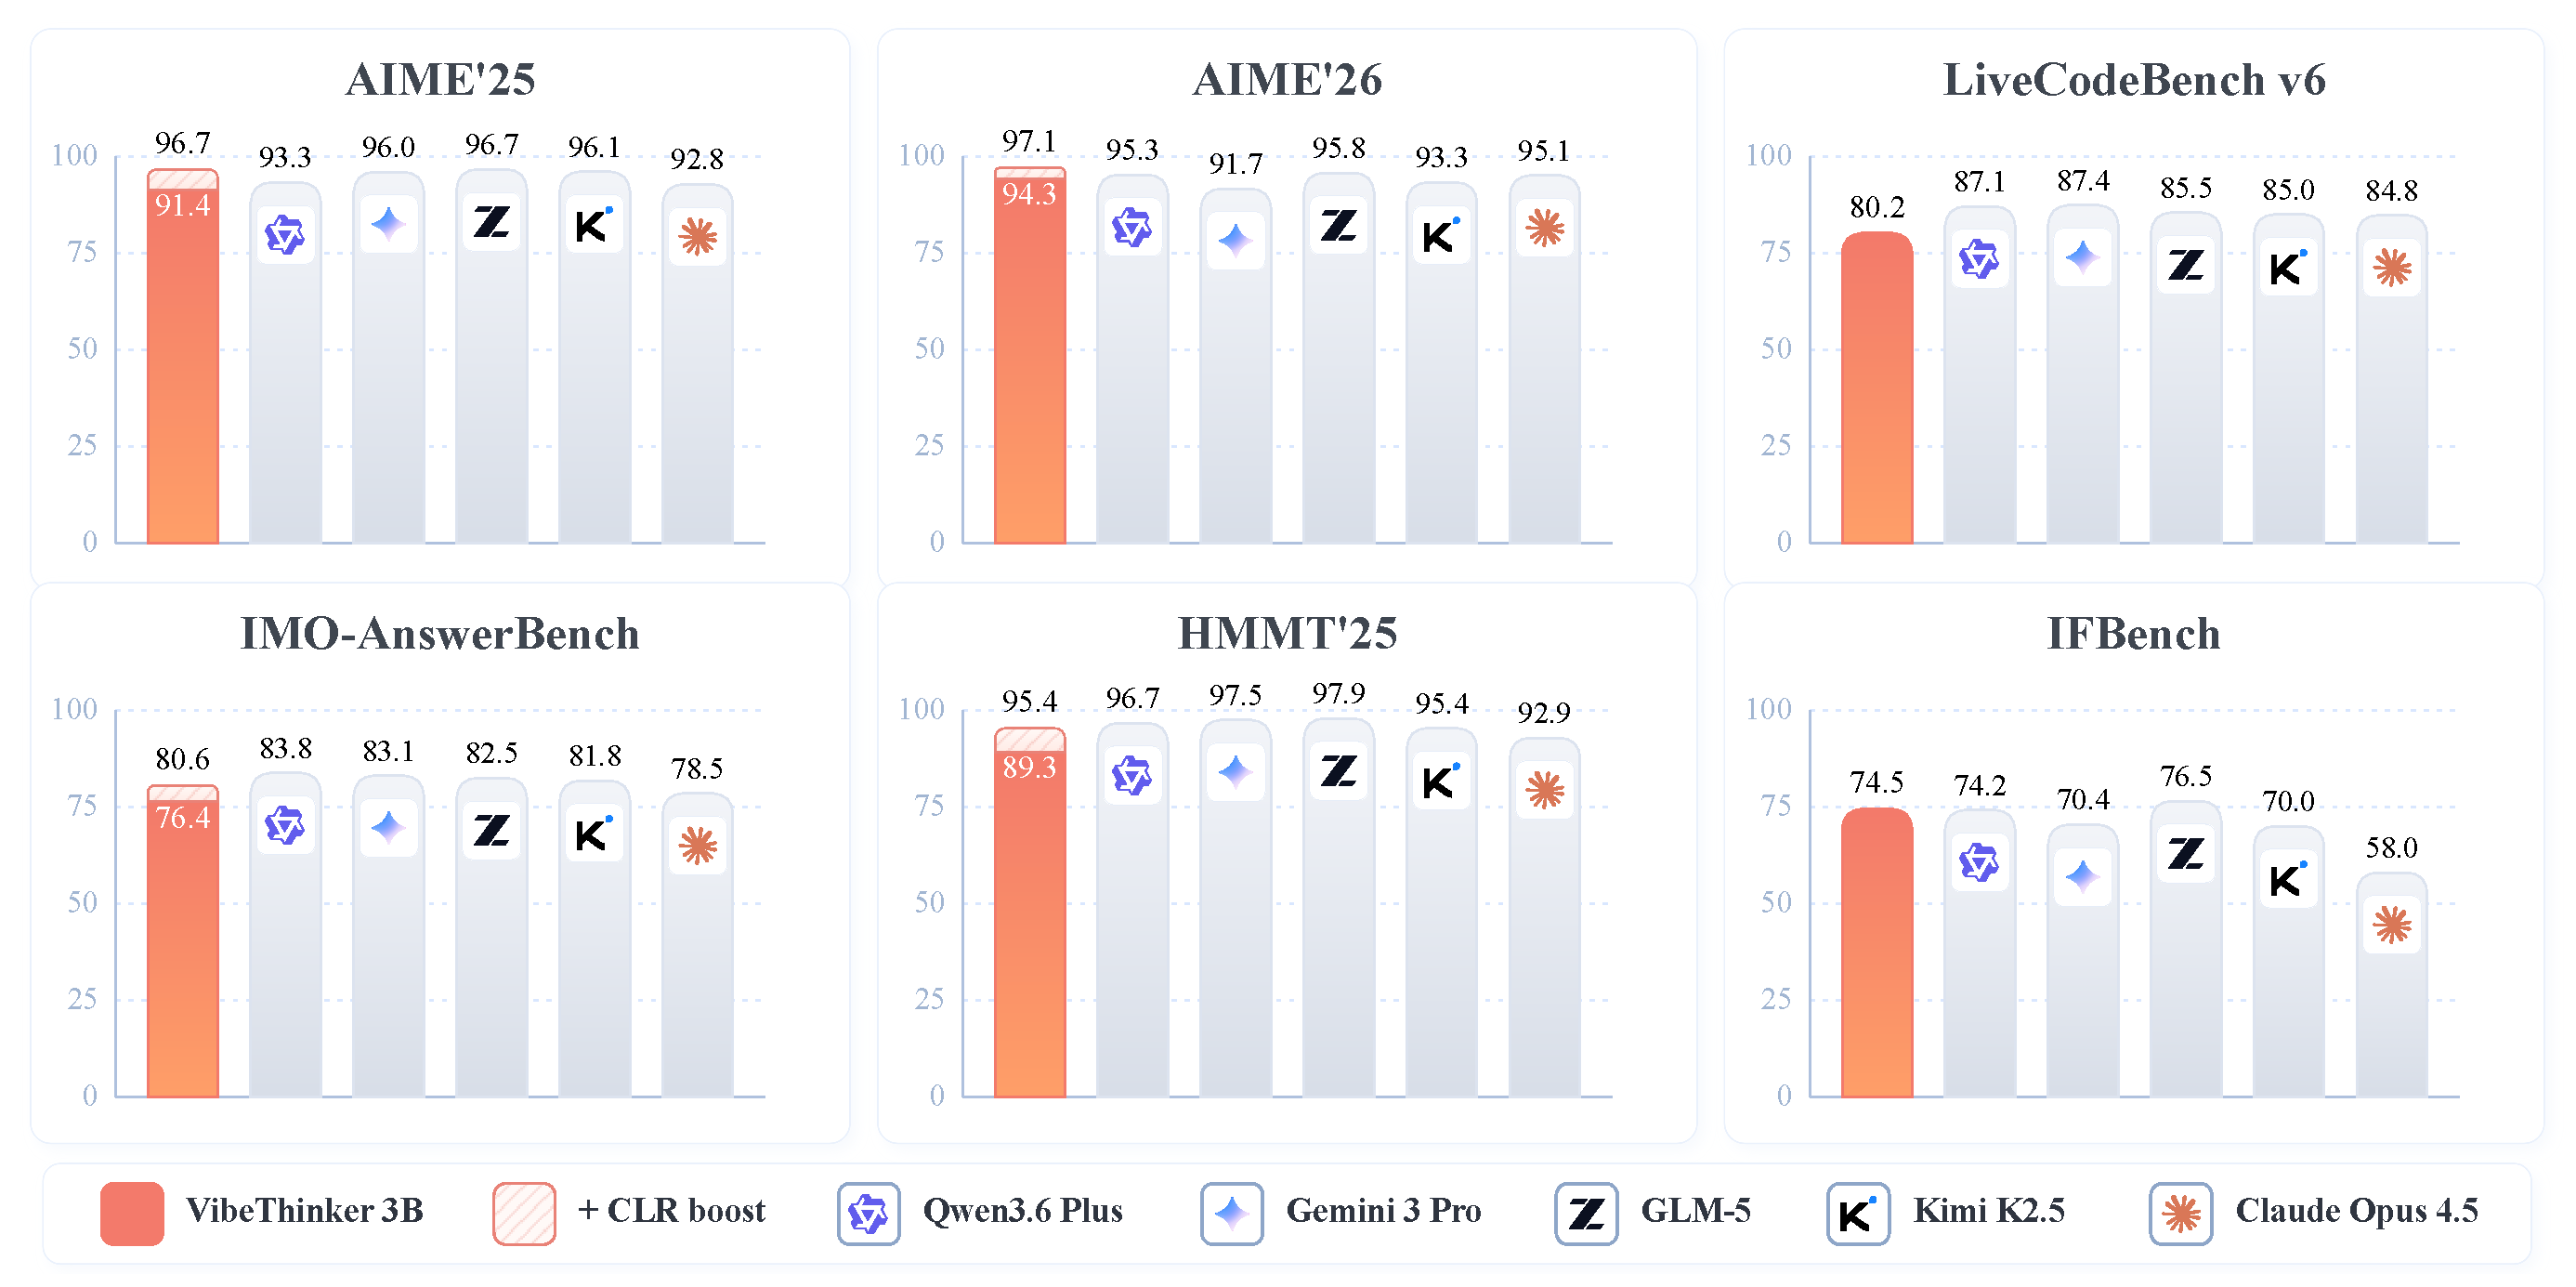
\includegraphics[width=0.98\textwidth]{image/v3_gai_legend_enhanced_reasoning_hero_vector.pdf}
\vspace{-1ex}
\caption{VibeThinker-3B는 3B 사이즈의 프론티어 뛰어난 성능을 발휘했습니다. CLR은 클레임 클래스 테스트 시간 축소 전략인 클레임 클래스 신뢰성을 평가합니다.}
    \label{fig:main-results}
\end{figure}

\begin{figure}[H]
\centering
    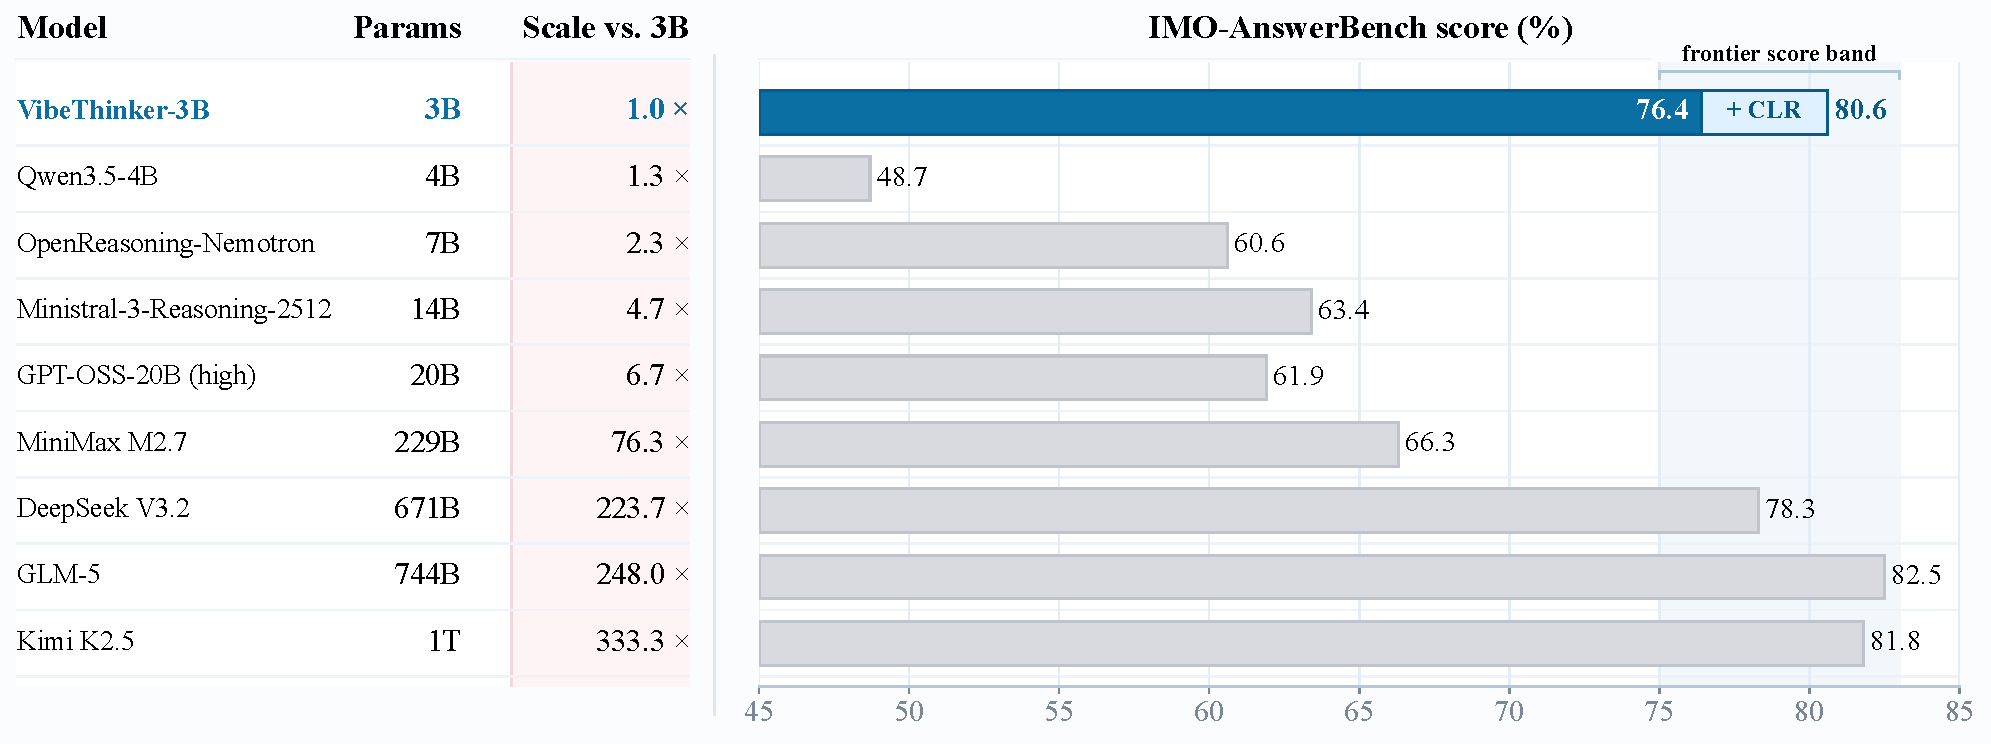
\includegraphics[width=0.92\textwidth]{image/frontier_gate_matrix_imo_answerbench.pdf}
\vspace{-1ex}
\caption{매개 가변형 오픈 소스 가능 모델 중 400개의 IMO 고급 문제로 매우 다루기 마크인 IMO-AnswerBench의 특정 가변 범위입니다. VibeThinker-3B는 3B 개별적으로 76.4를 배터리하고 CLR로 80.6에 접근하여 작은 모델을 보여줄 수 있도록 모델이 DeepSeek V3.2(78.3, 671B), GLM-5(82.5, 744B) 및 Kimi K2.5(81.8, 1T)와 같은 큰 모델의 성능에 초점을 맞출 수 있다는 것을 나타냅니다.}
    \label{fig:parameter-efficiency}
\end{figure}


\section{소개}


강화 학습~\cite{shao2024GRPO,yu2025dapo,zheng2025gspo,hu2025reinforce++}가 언어 모델의 학습 후 단계에 점점 더 통합됨에 따라 대형 모델의 복잡한 논리적 추론 능력이 크게 향상되었습니다. 현재 이 분야에서는 일반적으로 어려운 추론 작업에 필요한 임계값을 초과하기 위해 확장 법칙에 따라 매개변수 확장을 늘리는 데 의존합니다. 결과적으로 프론티어 추론 능력은 수백억 또는 수천억 개의 매개변수를 가진 모델에 집중되는 경우가 많습니다. 이와 대조적으로, 30억 개 이하의 매개변수를 갖는 소규모 언어 모델(SLM)은 배포 비용, 추론 효율성 및 학술 연구에 대한 광범위한 접근성 측면에서 분명한 이점을 제공하지만 일반적으로 어려운 수학적 파생 또는 복잡한 프로그래밍 작업을 처리할 때 내재된 병목 현상에 직면하는 것으로 간주됩니다.

VibeThinker-1.5B~\cite{xu2025vibethinker}에 대한 이전 작업에서는 매개변수 수가 극히 적은 모델이라도 안정적이고 기본적인 논리 체인을 생성하기 위해 도출될 수 있음을 보여주었습니다. 이는 작은 모델이 장기적인 추론에 어려움을 겪는다는 일반적인 믿음에 도전하려는 초기 시도였습니다. 그러나 1.5B 모델은 주로 작은 모델에서 추론의 타당성을 보여 주었지만 상한선은 아직 탐구되지 않았습니다. 이로 인해 추가 질문이 생겼습니다. \textbf{\textit{SLM을 단순히 계산 절약 폴백으로 처리하는 대신 실제 기능 경계는 무엇입니까? 엄격한 3B 모델이 실제로 최상위 LLM에 필적하는 최전선 수준의 성능을 달성할 수 있습니까?}} 따라서 이 보고서에서는 VibeThinker-3B에 대한 실증적 관찰을 제시하여 3B 규모에서 복잡하고 검증 가능한 추론의 한계를 추가로 조사합니다.

3B 모델의 추론 능력을 더욱 강화하기 위해 우리는 체계적으로
VibeThinker-1.5B에 도입된 스펙트럼-신호 원리를 기반으로 구축된 훈련 후 파이프라인을 업그레이드합니다. SFT 단계에서는 데이터 합성을 강화하고,
품질 필터링 및 커리큘럼 학습을 통해 모델이 먼저 획득할 수 있습니다.
수학, 코드, STEM, 일반 대화 및 교육 전반에 걸친 광범위한 범위
다음으로 더 어려운 장거리 추론 샘플에 집중하세요. RL에서는
단계에서는 MGPO~\cite{xu2025vibethinker}의 핵심 아이디어를 유지하면서 교육을 여러 단계로 확장합니다.
검증 가능한 도메인을 보존하고 보다 안정적인 장기 컨텍스트 전략을 채택합니다.
완전한 추론 궤적. Long2Short Math RL을 추가로 소개합니다.
희생하지 않고 중복 토큰을 줄여 추론 효율성을 향상시킵니다.
정확성. 마지막으로 오프라인 자체 증류와 Instruct RL이
여러 단계에서 도출된 역량을 통합 모델로 만들고 이를 개선합니다.
복잡하고 제약이 많은 사용자 지침에 따른 제어 가능성. 비교
VibeThinker-1.5B, VibeThinker-3B는 따라서 온건한 것뿐만 아니라
매개변수 규모가 증가할 뿐만 아니라 보다 완벽한 사후 훈련 시스템도 제공됩니다.
역량 구축, 추론 증폭, 효율성을 공동으로 해결
최적화 및 명령어 정렬.

엄격한 데이터 오염 제거 하에 여러 독립 경쟁 시스템에 대한 광범위한 평가를 통해 VibeThinker-3B의 탁월한 매개변수 효율성이 확인되었으며 우리의 결과가 단일 벤치마크에 국한되지 않는지 확인되었습니다. 기존 중소형 추론 모델보다 지속적으로 뛰어난 성능을 발휘하지만, 가장 중요한 성과는 수십 배 더 큰 최상위 시스템에 대한 경쟁력을 입증한 것입니다. 3B 매개변수만 있음에도 불구하고 VibeThinker-3B는 AIME26~\cite{maa2026aime}에서 94.3점을 달성하여 DeepSeek V3.2~\cite{liu2025deepseekv3.2}(671B) 및 Kimi K2.5~\cite{team2026kimik2.5}(1T)와 같은 훨씬 더 큰 모델의 성능과 일치합니다. 또한 HMMT25~\cite{hmmt2025}에서 89.3점을 얻었고 LiveCodeBench~\cite{jain2024livecodebench} v6에서 80.2 Pass@1을 달성하여 GPT-OSS-120B 및 DeepSeek V3.2의 성능에 바짝 뒤처졌습니다. 또한 테스트 시간 확장 전략인 CLR(클레임 수준 신뢰성 평가)을 사용하여 답변 검증 가능한 수학 벤치마크에서 추가 이득을 얻어 AIME26 점수를 97.1로, HMMT25를 95.4로, BruMO25~\cite{brumo2025}를 99.2로 높였습니다. VibeThinker-3B는 표준 벤치마크를 넘어서 강력한 배포 외 일반화를 보여 최근 LeetCode 주간 및 격주 콘테스트(2026.04.25~2026.05.31)에서 96.1\% 승인률을 달성했습니다. 이는 GPT-5.2~\cite{openai2025gpt52systemcard} 및 Gemini 3와 같은 업계 최고의 모델과 비교할 수 있는 합격률 수준입니다. 플래시~\cite{googledeepmind2025gemini3flashmodelcard}.
VibeThinker 시리즈의 기술 계보를 확장한 이러한 성과는 엄격한 3B 매개변수 예산이 Gemini 3 Pro, GLM-5 및 Kimi K2.5와 같은 주요 추론 모델의 성능 범위에 접근하는 데 전적으로 충분하다는 것을 보여 주며, 소형 모델의 추론 용량 한계가 기존 기대치를 훨씬 뛰어넘는다는 것을 증명합니다.


% Extending the technical lineage of the VibeThinker series, VibeThinker-3B is designed to explore the boundaries of reasoning capacity within SLMs. Rather than pursuing broad open-domain generalism, we investigate the extent to which highly demanding verifiable tasks, such as mathematics and coding, can be pushed while the model scale remains strictly within a compact regime. Experimental results demonstrate that the 3B parameter budget is entirely sufficient to sustain highly intensive algorithmic and mathematical computations. Across multiple benchmarks, it approaches the performance of top-tier systems such as Gemini 3 Pro, GLM-5, and Kimi K2.5. This finding compellingly illustrates that the reasoning depth of small models far exceeds conventional expectations.

% The primary objective of VibeThinker-3B is not to construct a compact model as comprehensive as large-parameter generalist models. Instead, building upon the trajectory established by VibeThinker-1.5B, it aims to further probe the extreme depth limits of small models in verifiable reasoning through optimized post-training methodologies. In other words, our focus is neither on whether small models can immediately supplant flagship generalist models, nor on their practical upper bounds across all open-domain tasks. Rather, we investigate the extent to which highly demanding verifiable reasoning capabilities, such as mathematics and coding, can be pushed while the model scale remains strictly within a compact regime. Experimental results demonstrate that the 3B parameter scale is entirely sufficient to sustain highly intensive mathematical and algorithmic reasoning computations. Across multiple verifiable tasks, it approaches the performance of top-tier systems such as Gemini 3 Pro, GLM-5, and Kimi K2.5. This finding compellingly illustrates that the depth boundary of reasoning capabilities in small models may far exceed conventional expectations.


이러한 발견에 동기를 부여하여 우리는 기본 모델 기능이 필요한 매개변수 용량의 양뿐만 아니라 매개변수 요구의 구조적 형태에서도 다르다는 것을 가정하는 매개변수 압축 범위 가설을 소개합니다. 이러한 관점에서 보면 매개변수 밀도 기능과 매개변수 확장 기능으로 크게 나눌 수 있습니다. 검증 가능한 추론은 전자를 예시합니다. 핵심 과제는 방대한 공개 도메인 사실을 기억하는 것이 아니라 구조화된 솔루션 공간 내에서 검색, 제약 조건 충족, 오류 수정 및 다단계 구성을 수행하는 데 있습니다. 결과적으로 이 클래스는 컴팩트하고 재사용 가능한 추론 코어로 고도로 압축될 수 있습니다. 이와 대조적으로, 지식 집약적 및 범용 능력은 개방형 도메인 사실, 도메인별 개념, 의미 체계 연관 및 롱테일 시나리오에 대한 광범위한 범위를 요구하므로 후자와 더 밀접하게 일치합니다. 따라서 그들의 매개변수 요구는 재사용 가능한 추론 코어의 압축보다는 적용 범위 문제와 유사합니다. 이러한 관점은 VibeThinker-3B가 GPQA-Diamond와 같은 지식 집약적 벤치마크에서 더 큰 모델에 비해 여전히 격차를 보이는 동시에 수학 및 코딩과 같은 검증 가능한 작업에서 최상위 시스템에 필적하는 성능을 달성하는 이유를 설명합니다.

매개변수 스케일링은 광범위한 모델 기능의 기본 동인으로 남아 있지만, 우리는 더 작은 모델의 고도로 전문화된 잠재력을 드러내기 위해 추론-지식 분리 패러다임을 제안합니다. 이 패러다임 하에서 대규모 모델은 다양한 의미론과 롱테일 분포를 흡수하려면 본질적으로 대규모 매개변수 용량이 필요하기 때문에 광범위한 지식 폭을 위한 자연스러운 수단 역할을 계속합니다. 반대로, 구조적으로 제한된 공간과 신뢰할 수 있는 훈련 신호가 제공되면 더 작은 모델로도 이미 고밀도 추론 깊이를 캡슐화하는 데 충분합니다. 따라서 VibeThinker-3B의 진정한 의미는 3B 모델이 대규모 일반 작업자를 대체할 수 있다는 것을 증명하는 데 있는 것이 아니라 구체적인 경험적 신호를 제공하는 데 있습니다. 컴팩트 모델의 개발은 더 이상 배포 효율성이나 비용 제어를 위한 수동적인 타협이 아닙니다. 이는 전통적인 매개변수 스케일링 패러다임을 근본적으로 보완하는 유망한 연구 궤도로 떠오릅니다.

% Based on these findings, we introduce a more heuristic analytical perspective: when evaluating model capabilities, it is highly beneficial to conceptually decouple the "knowledge storage load" from the "reasoning computation load" borne by the parameters. Large-scale parameters retain a significant advantage in encoding massive open-domain knowledge and supporting complex, general-purpose scenarios that demand a broad spectrum of capabilities. This is objectively reflected in the performance gap between VibeThinker-3B and its large-parameter counterparts on knowledge-intensive benchmarks such as GPQA-Diamond. 


% Therefore, the true significance of VibeThinker-3B does not lie in proving that a 3B model can replace generalist flagships, but rather in providing a concrete empirical signal: for verifiable reasoning tasks, expert-level logical computation capabilities can be compressed into a parameter scale vastly smaller than that of traditional flagships. Consequently, the pursuit of small models is no longer merely a passive compromise for deployment efficiency or cost control; it emerges as a promising research trajectory that is fundamentally complementary to the traditional parameter scaling paradigm.



\begin{figure}[t]
\centering
    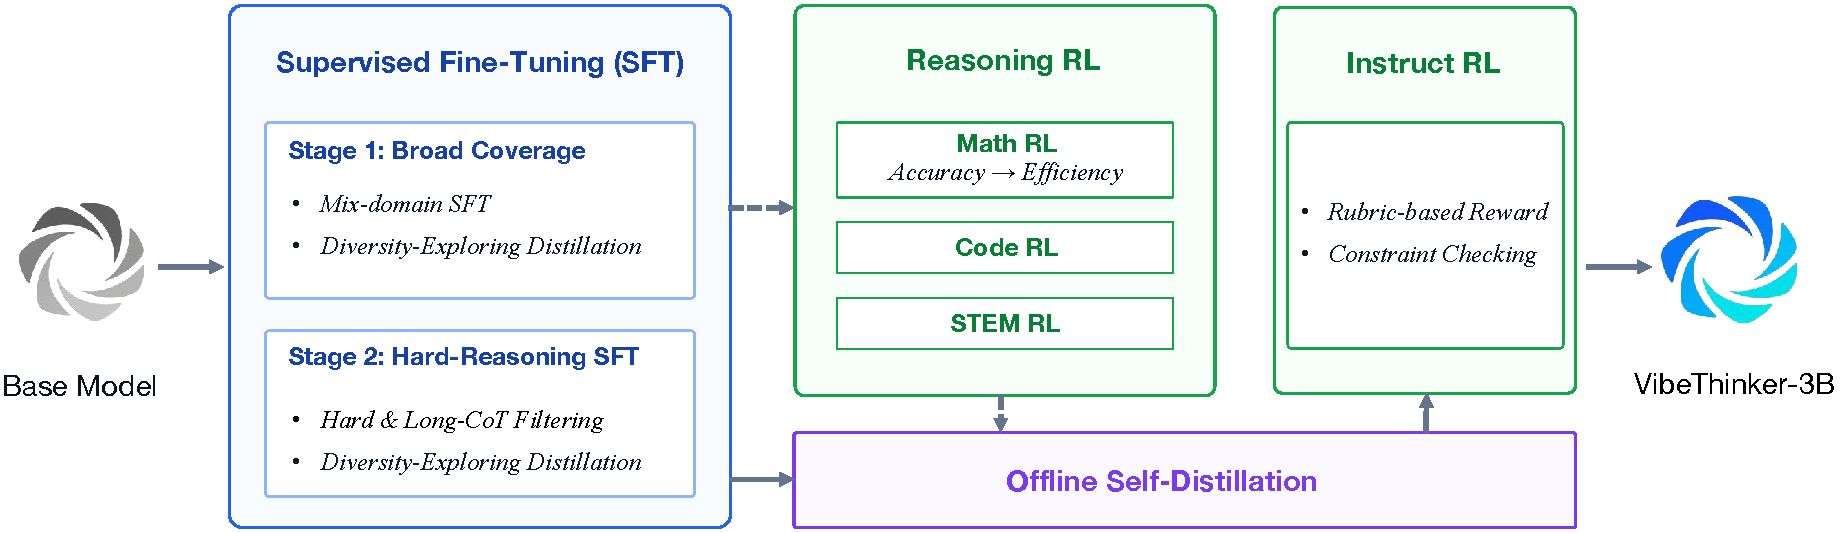
\includegraphics[width=\textwidth]{./image/overall_pipeline.pdf}
\caption{VibeThinker-3B의 전체 파이프라인.}
    \label{fig1:pipeline}
\end{figure}

\section{ 행동 양식}

\textbf{전체 파이프라인.} VibeThinker-3B는 소형 3B 밀도 기반 모델인 Qwen2.5-Coder-3B 기반을 기반으로 구축된 단계적 사후 훈련 파이프라인을 통해 개발되었습니다. 우리의 초점은 데이터 합성, 다양성 중심 지도 미세 조정, 다중 영역 강화 학습, 오프라인 자체 증류 및 교육 중심 정렬을 통해 추론 능력을 체계적으로 도출하고 통합하는 데 있습니다. 전체 사후 훈련 프레임워크는 VibeThinker-1.5B ~\cite{xu2025vibethinker}에 도입된 \textit{스펙트럼-신호 원리(SSP)}를 계속합니다. 이전 작업의 핵심 방법론을 기반으로 SFT 단계에서 다양성 탐색 증류를 계속 사용하여 광범위한 솔루션 공간("스펙트럼")을 구축하고, RL 단계에서 MaxEnt-Guided Policy Optimization(MGPO)을 활용하여 고가치 추론 신호("신호")를 증폭합니다.

이번 3B 반복을 위해 우리는 원래 기반을 기반으로 데이터 구성 및 전체 교육 파이프라인을 포괄적으로 최적화했습니다. 그림 \ref{fig1:pipeline}에 묘사된 것처럼 완전한 사후 훈련 프레임워크는 단계적으로 순차적으로 전개됩니다. 첫째, SFT(Supervised Fine-Tuning) 단계에서는 엄격한 데이터 합성 및 필터링 파이프라인을 업그레이드하여 2단계 커리큘럼 학습 전략 도입을 지원합니다. 이를 통해 모델은 광범위한 기능 범위에서 심층적이고 장기적인 추론으로 원활하게 전환할 수 있습니다. 그 후 강화 학습(RL) 단계에서는 크게 확장된 컨텍스트 창을 활용하여 다중 도메인 추론 작업에 MGPO를 적용합니다. 또한 수학적 RL 단계에서는 정확성을 저하시키지 않고 추론 효율성을 최적화하도록 설계된 Long2Short 단계를 도입합니다. 핵심 추론 RL이 완료된 후 파이프라인은 즉시 오프라인 자체 증류 단계로 진행하여 새로 도출된 기능을 백피드하고 마지막으로 Instruct RL 단계로 마무리하여 복잡한 다단계 지침에 대한 모델의 엄격한 준수를 더욱 강화합니다. 후속 하위 섹션에서는 각 단계의 세부 구현을 체계적으로 설명합니다.



\subsection{감독된 후 조정}

\subsubsection{데이터 구축}

SFT 단계에서는 기본 모델을 기반으로 다중 도메인 혼합 감독 데이터 세트를 구성하여 후속 RL 단계에 안정적인 콜드 스타트 ​​정책을 제공합니다. 데이터세트에는 수학, 코드, STEM 추론, 일반 채팅, 지침 따르기 등 다양한 작업이 포함됩니다.

\textbf{데이터 합성 및 쿼리 확장.} VibeThinker-3B는 훈련 쿼리의 적용 범위를 넓히기 위해 SFT 단계에서 자동화된 데이터 합성 파이프라인을 도입합니다. 기존 데이터세트에서 신뢰할 수 있는 감독 신호가 있는 쿼리만 시드 쿼리로 선택합니다. 수학적 쿼리에는 명시적이고 신뢰할 수 있는 최종 답이나 해결 근거가 있어야 하며, 경쟁력 있는 프로그래밍 쿼리에는 신뢰할 수 있는 단위 테스트 또는 실행 가능한 평가 규칙이 갖추어져 있어야 합니다. 이러한 신뢰도가 높은 시드 샘플을 기반으로 개념 구성, 문제 해결 골격, 제약 조건, 평가 목표 등 여러 차원에 걸쳐 쿼리를 다시 작성하고 확장하여 더 넓은 범위의 지식 구성과 추론 패턴을 포괄하는 파생 쿼리를 생성합니다. 초기에 필터링된 합성 쿼리의 경우 강력한 교사 모델을 사용하여 여러 개의 독립적인 샘플링을 추가로 수행하고 다수 투표를 통해 의사 레이블을 생성하여 후속 증류 및 훈련을 위한 기반을 구축합니다.

\textbf{다중 경로 추론 증류.} 수학, 코드 및 STEM의 추론 집약적 샘플을 위해 다중 경로 증류 접근 방식을 채택하여 SFT 응답을 구성합니다. 특히 우리는 강력한 교사 모델을 사용하여 각 쿼리에 대해 여러 후보 추론 추적을 샘플링하고 단일 표준 솔루션만 유지하는 대신 전체 중간 추론 단계를 유지합니다. 이 설계는 VibeThinker-1.5B의 스펙트럼-신호 패러다임을 상속하여 SFT 단계가 다양한 유효한 방법을 포괄하는 솔루션 스펙트럼을 구성하고 후속 RL을 위한 더 넓은 후보 솔루션 공간을 제공하는 임무를 맡습니다. 이 다중 솔루션 구조를 명시적으로 보존함으로써 모델은 다양한 분해 방법, 파생 경로 및 검증 전략을 학습하여 후속 정책 샘플링 중에 탐색 다양성을 향상시킵니다.

\textbf{다단계 품질 관리.} SFT 데이터의 품질은 후속 RL의 성능 상한을 직접적으로 결정합니다. 결과적으로 우리는 보다 엄격한 다단계 품질 관리 프로세스를 구현합니다.
\begin{itemize}
\item \textit{1). N-그램 기반 필터링.} 품질이 낮은 생성 및 벤치마크 오염을 제거하기 위해 비정상적인 반복 세그먼트, 템플릿 변질 패턴 또는 평가 세트와 n-그램 중복이 포함된 샘플을 폐기합니다.
\item \textit{2). LLM 기반 쿼리 품질 필터링.} 우리는 유능한 LLM을 활용하여 쿼리 품질을 평가하고 불완전한 설명, 불합리한 조건, 유효하지 않은 논리 또는 대상 지식 포인트를 효과적으로 평가할 수 없는 샘플을 필터링합니다.
\item \textit{3). 추적 정확성 필터링.} 증류된 응답 수준에서는 답변 확인, 코드 샌드박스 실행 및 LLM 다수결 투표의 조합을 통해 추론 추적을 검사합니다. 잘못된 최종 답변, 실패한 실행 결과 또는 명백히 유효하지 않은 추론 단계가 있는 추적은 필터링됩니다.
\end{itemize}
그런 다음 품질 관리 데이터는 추론 체인 길이와 문제 난이도에 따라 계층화되어 후속 커리큘럼 SFT를 위한 데이터 기반을 구축합니다.

\subsubsection{훈련 과정}

\textbf{커리큘럼 기반 2단계 SFT 전략.} VibeThinker-1.5B와 비교하여 VibeThinker-3B는 커리큘럼 기반 2단계 SFT 절차를 채택합니다. 첫 번째 단계에서는 광범위한 기능 적용 범위와 동작 콜드 스타트에 중점을 둡니다. 우리는 작업 유형과 추론 패턴의 다양성을 극대화하기 위해 전체 품질 필터링 추론 데이터 세트를 훈련에 활용합니다. 첫 번째 단계 데이터 내에서 CoT(사고 사슬) 길이의 상당한 차이를 고려하여 훈련 효율성을 높이기 위해 시퀀스 패킹을 사용합니다. 최적화를 위해 전역 배치 크기 128을 사용하고 초기 학습 속도를 $5\times10^{-5}$로 설정했습니다. 학습률은 코사인 어닐링 일정을 따르며 최소값 $8\times10^{-8}$로 감소합니다. 첫 번째 단계는 5\% 선형 워밍업을 통해 5세대 동안 학습됩니다.

안정적이고 광범위한 SFT 모델을 획득하면 두 번째 단계로 진행하여 훈련 데이터 분포를 더 어렵고 더 긴 지평선 추론 샘플로 이동합니다. 첫 번째 단계의 마지막 체크포인트부터 초기화된 이 단계는 관절 길이 난이도 필터링을 통해 생성된 하드 추론 하위 집합에 대한 훈련을 계속합니다. 구체적으로, 먼저 추론 추적이 5,000개 토큰보다 짧은 샘플을 삭제합니다. 이후 VibeThinker-1.5B를 참조 모델로 사용하여 쿼리당 8개의 독립적인 롤아웃을 수행하여 오류율이 0.75 미만인 비교적 쉬운 문제를 필터링합니다. 이 필터링 전략은 얕은 추론 데이터의 비율을 효과적으로 줄여 2단계 SFT가 장거리 논리적 파생, 복잡한 제약 조건 만족 및 고급 문제 해결에 집중하도록 합니다. 첫 번째 단계의 정확한 하이퍼파라미터 구성을 유지하면서 이 단계에서는 하드 샘플 하위 집합에 대해 추가로 2번의 훈련을 거칩니다.

\textbf{Diversity-Exploring Distillation.} VibeThinker-1.5B~\cite{xu2025vibethinker}에 이어 두 SFT 단계 모두에 Diversity-Exploring Distillation을 적용하여 다중 도메인 훈련에서 잠재적인 경사 간섭을 완화하고 모델 출력의 추론 다양성을 보존합니다. 이 방법은 스펙트럼-신호 원리를 따릅니다. SFT 단계는 단일 솔루션 경로를 따라 최적의 모방을 목표로 하지 않고 대신 더 넓은 후보 솔루션 공간의 구성에 우선 순위를 두어 후속 RL에 대한 더 풍부한 탐색 기반을 제공합니다.

특히 훈련 중에 중간 체크포인트를 주기적으로 저장하고 도메인별 프로브 세트에서 Pass@K 성능을 평가합니다. 각 도메인에 대해 단순히 검증 손실이 가장 낮거나 Pass@1이 가장 높은 체크포인트를 선택하는 것이 아니라 더 유효한 솔루션을 생성하는 체크포인트를 해당 전문가 모델로 선택합니다. 이러한 도메인 전문가 모델은 매개변수 수준에서 병합되어 통합 SFT 모델을 얻습니다. 결과 병합 모델은 높은 출력 다양성을 유지하면서 도메인별 추론 기능을 유지하므로 후속 교육 단계에 더 넓은 솔루션 스펙트럼을 제공합니다.

\subsection{강화 학습}
% \subsubsection{Reasoning RL}
\subsubsection{알고 백본}

VibeThinker-1.5B~\cite{xu2025vibethinker}에 도입된 MGPO(MaxEnt-Guided Policy Optimization)를 핵심 RL 알고리즘으로 재사용합니다. 스펙트럼-신호 원리에 따라 SFT는 다양한 솔루션 공간을 구성하고 RL은 그 안에서 올바른 추론 신호를 증폭하는 역할을 담당합니다. MGPO는 모델의 현재 기능 경계 근처에 있는 프롬프트를 동적으로 선택하여 이 역할을 수행합니다.

각 프롬프트 $q$에 대해 이전 정책에서 $G$ 응답을 샘플링하고 검증 가능한 보상으로 평가합니다. 경험적 그룹 정확도는 다음과 같이 계산됩니다.
\begin{equation}
p(q)=\frac{1}{G}\sum_{i=1}^{G}\mathbb{I}(r_i=1).
\end{equation}

$p(q)\approx 0$가 포함된 프롬프트는 너무 어렵고 희박한 긍정적인 신호를 제공하는 반면, $p(q)\approx 1$가 포함된 프롬프트는 이미 포화 상태입니다. 따라서 MGPO는 중간 정도의 정확성을 지닌 프롬프트에 더 높은 가중치를 할당합니다.
\begin{equation}
w(q)=\exp\left(-\gamma D_{\mathrm{ME}}(\,p(q)\,\|\,p_0\,)\right),\quad \mathrm{여기서}\,\, p_0 = 0.5,\, \gamma > 0.
\end{equation}

여기서 $D_{\mathrm{ME}}(p(q)\|p_0)$는 경험적 정확성 $p(q)$가 최대 엔트로피 지점 $0.5$에서 얼마나 벗어나는지 측정합니다. 값이 작을수록 프롬프트가 올바른 롤아웃과 잘못된 롤아웃이 공존하는 모델의 현재 기능 경계에 더 가깝다는 것을 나타냅니다. 이 가중치는 GRPO 스타일 클립 목표 내부의 그룹 상대적 이점에 적용됩니다.
\begin{equation}
\mathcal{J}_{\mathrm{MGPO}}(\theta)
=
\mathbb{E}_{q,\{y_i\}}
\!\left[
\frac{1}{G}\sum_{i=1}^{G}
\frac{1}{|y_i|}\sum_{t=1}^{|y_i|}
\min\!\bigl(
\rho_{i,t}(\theta)\,w(q)A_i,\;
\mathrm{클립}(\rho_{i,t}(\theta),1\!-\!\varepsilon,1\!+\!\varepsilon)\,w(q)A_i
\bigr)
\right]\!,
\end{equation}

여기서 $A_i$는 그룹 상대 우위, $\rho_{i,t}(\theta)$는 현재 정책과 기존 정책 간의 토큰 수준 확률 비율, $\varepsilon$는 클리핑 계수입니다. 최대 엔트로피 원리에서 영감을 받은 이 가중치 메커니즘은 RL 업데이트가 불확실성이 충분한 프롬프트에 집중하도록 장려하여 보다 안정적이고 건강한 기울기 신호를 생성합니다. 또한 확률이 높은 토큰에 대한 과도한 최적화를 완화하고 정책 업데이트 중 시끄러운 토큰의 부정적인 영향을 줄입니다.


VibeThinker-3B에서는 핵심 MGPO 공식을 변경하지 않고 유지하면서 훈련 안정성을 향상시키기 위해 몇 가지 조정을 수행했습니다. 훈련 중에 롤아웃 엔진이 추론 처리량에 대해 점점 더 최적화됨에 따라 훈련-추론 확률 불일치가 여러 구현 요소에 의해 점차 증폭되는 것을 관찰했습니다. 이러한 불일치로 인해 RL 훈련이 불안정해지거나 심지어 붕괴될 수도 있습니다. 이 문제를 완화하기 위해 우리는 ~~\cite{fangkhazi2025mismatch,yao2025mismatch}의 안정화 전략을 채택하고 모든 RL 단계를 정책에 따라 수행합니다.

\subsubsection{다중 처리 RL}

우리는 수학, 코드 및 STEM 추론을 포함한 다중 도메인 검증 가능한 추론 작업에 MGPO를 적용합니다. 이러한 도메인은 동일한 정책 최적화 프레임워크를 공유하지만 서로 다른 보상 소스와 확인 메커니즘을 사용합니다. 수학적 작업은 주로 최종 답변 확인에 의존하고, 코드 작업은 샌드박스 실행 및 테스트 사례에 의존하며, STEM 작업은 답변 일치와 옵션 확인을 결합합니다.

\textbf{훈련 데이터.} 모든 도메인에 대해 훈련 세트는 신뢰할 수 있는 감독 신호가 있는 데이터로 구성되며 엄격한 벤치마크 오염 제거를 거쳤습니다. 또한 훈련이 시작되기 전에 각 단계의 시작 체크포인트에서 평가한 대로 정확히 0.0 또는 1.0의 정확도를 산출하는 샘플을 필터링합니다.

\textbf{단일 장기 컨텍스트 학습.} ~\cite{luo2025deepscaler}는 점진적인 컨텍스트 창 확장을 기반으로 하는 다단계 RL 전략을 도입하여 훈련 효율성과 최종 추론 성능을 모두 향상시킵니다. 우리는 VibeThinker-1.5B에서도 유사한 현상을 관찰했는데, 컨텍스트 창을 점진적으로 확장하면 더 낮은 훈련 비용으로 더 나은 추론 성능을 얻을 수 있었습니다.

그러나 이 결론은 VibeThinker-3B에서는 적용되지 않습니다. 우리는 높은 절단 초기 단계가 모델의 장기적인 사고 능력을 약화시키고 정책이 불완전하거나 과도하게 단축된 추론 궤적 쪽으로 편향된다는 것을 발견했습니다. 우리는 이러한 반전이 더 강력한 RL 초기화 체크포인트와 관련이 있다고 가정합니다. VibeThinker-1.5B와 비교하여 VibeThinker-3B는 더 엄격한 SFT 데이터 품질 제어를 거치고 유효하지 않은 추론 패턴이 더 적습니다. 결과적으로 잘림이 많은 워밍업은 더 이상 시끄러운 사고 흔적을 주로 제거하지 않고 대신 기존의 고품질 장거리 추론 동작을 방해할 수 있습니다. 나중에 컨텍스트 창이 확장된 후에도 이러한 저하를 완전히 복구하기는 어렵습니다. 따라서 우리는 단일 64K 긴 컨텍스트 창으로 RL을 직접 수행하여 롤아웃 잘림을 줄이고 긴 수평 추론 궤적을 더 잘 보존합니다.


\textbf{Training Strategy.} 그림 \ref{fig1:pipeline}에 설명된 대로 순차적 다중 도메인 추론 RL 파이프라인을 채택합니다. 훈련은 모델의 장거리 기호 파생, 복잡한 조건 구성 및 다단계 검색 기능을 강화하는 Math RL로 시작됩니다. 그런 다음 실행 가능한 논리의 엄격함, 경계 사례 처리 및 프로그램 제약 조건 만족을 개선하는 데 중점을 두고 Code RL로 원활하게 전환됩니다. 마지막으로, 우리는 STEM RL을 수행하여 기본 논리적 추론 능력을 다학문적 과학 시나리오로 일반화하고 지식 활용 및 교차 도메인 추론을 향상시킵니다. 각 RL 단계 후에 얻은 체크포인트는 보존되어 후속 \textbf{\textit{오프라인 자체 증류 단계}}에서 사용됩니다. 여기서 다양한 단계에서 도출된 고품질 추론 궤적이 수집되어 모델의 전체 추론 기능을 더욱 통합합니다.

\textbf{Long2Short Math RL.} 이전 작업과 달리 VibeThinker-3B는 \textbf{\textit{'정확도에서 효율성까지'}} 2단계 강화 학습 전략을 채택합니다. 첫 번째 단계에서는 표준 MGPO를 사용하여 정확도를 최적화하여 모델이 추론 프로세스를 완전히 펼치고 다양한 솔루션 경로를 탐색할 수 있도록 합니다. 이어서 Math RL에 Long2Short 단계를 도입하여 최적화 목표를 순수한 정확도 향상에서 토큰 효율성 최적화로 확장합니다. 이 단계의 목표는 검증 세트 성능을 유지하면서 중복 추론을 줄이고 출력 효율성을 높이는 것입니다.
Long2Short RL에서는 응답 길이에 따라 각 프롬프트 그룹의 올바른 궤적 간에만 보상을 재분배하여 더 짧은 정답에 대한 보상을 늘리고 긴 정답에 대한 보상을 줄입니다. 샘플링된 각 궤적 $y_i$에 대해 이진 정확성 보상 $r_i\in\{0,1\}$를 얻은 후 모든 잘못된 궤적을 변경하지 않고 유지합니다. 올바른 세트 $\mathcal{C}=\{i\mid r_i=1\}$에 대해 간결성 점수 $s_i=1/L_i$를 정의합니다. 여기서 $L_i$는 응답 길이를 나타내고 중심 길이 인식 보상 이동을 적용합니다.
\[
r_i' = r_i + \lambda \cdot
\frac{s_i-\bar{s}}{\max_{j\in\mathcal{C}} |s_j-\bar{s}|},
\qquad i\in\mathcal{C},
\]
여기서 $\bar{s}$는 올바른 궤적에 대한 평균 간결성 점수이고 0.2로 설정된 $\lambda$는 최대 재분배 크기를 제어합니다. 모든 올바른 궤적의 길이가 동일한 경우 보상은 변경되지 않습니다. 보상 변화는 $\mathcal{C}$ 내 중심에 있으므로 그 합은 0입니다.
\[
\sum_{i\in\mathcal{C}}(r_i'-r_i)=0.
\]
따라서 재분배 전후의 평균 보상은 올바른 하위 집합에 대해 변경되지 않고 유지되며, 잘못된 보상도 변경되지 않으므로 전체 프롬프트 그룹에 대해 변경되지 않습니다. 이 제로섬 설계는 이점 추정에 사용되는 그룹 수준 보상 기준에 대한 체계적인 이동을 방지하는 동시에 올바른 궤적 간의 상대적 선호도를 보다 간결한 추론 경로로 재구성합니다.


\subsection{오프라인에 접근하는 방법}

다중 도메인 Reasoning RL을 완료한 후 데이터 필터링과 함께 Math, Code 및 STEM RL 단계의 체크포인트를 사용하여 고품질 추론 패턴이 포함된 오프라인 궤적을 추출합니다. 그런 다음 이러한 궤적은 감독된 미세 조정을 통해 통합 학생 모델로 다시 증류되어 다중 영역 추론 기능을 보다 안정적으로 통합할 수 있습니다.

\textbf{Learning-potential Filtering.} 먼저 도메인별 검증기로 거부 샘플링을 수행하여 잘못된 궤적을 제거합니다. 검증된 교사 궤적을 얻은 후 학생 모델에 대한 각 올바른 추적의 증류 값을 추정하기 위해 학습 잠재력 점수를 추가로 도입합니다. 특히 입력 $q$와 검증된 교사 궤적 $y$에 대해 학생 모델에서 길이 정규화 음의 로그 가능성을 계산합니다.
\begin{equation}
S_{\mathrm{LP}}(q,y)
=
-\frac{1}{|y|}
\sum_{t=1}^{|y|}
\log \pi_{\theta_{\mathrm{stu}}}(y_t \mid q,y_{<t}).
\end{equation}
점수가 높을수록 교사가 추적을 성공적으로 생성하고 확인했지만 학생이 아직 잘 모델링하지 않았으므로 증류 가치가 더 높다는 것을 의미합니다.

이 점수가 시퀀스 길이나 비정상적인 토큰으로 인해 편향되는 것을 방지하기 위해 추적의 순위를 전체적으로 지정하지 않습니다. 대신, 도메인별 길이 버킷 내에서 우선순위를 계산합니다. 매우 짧은 추적은 점수 기반 선택에서 제외됩니다. 평균 점수가 몇 가지 비정상적인 토큰에 의해 지배될 수 있기 때문입니다. 또한 매우 높은 점수를 받은 이상값을 필터링하여 형식 오류, 분포 변화 또는 노이즈가 있는 샘플의 영향을 줄입니다. 마지막으로 중간에서 높은 점수 범위에서 검증된 추적의 우선순위를 지정하고 선택한 데이터를 수학, 코드 및 STEM 전반에 걸쳐 혼합하여 오프라인 자가 증류 데이터 세트를 구성합니다.

\subsection{RL에게 위험하기}

마지막으로 Instruct RL을 적용하여 추론 강화 체크포인트를 보다 안정적인 사용자 지향 모델로 변환합니다. 형식에 민감한 프롬프트, 긴 컨텍스트 지침 및 일반 정렬 예가 포함된 혼합 지침 데이터 세트를 교육합니다. 명시적인 제약 조건이 있는 샘플의 경우 형식, 순서, 항목 수, 키워드 제약 조건 및 작업 완료를 확인하는 규칙 기반 유효성 검사기에 의해 보상이 계산됩니다. 개방형 프롬프트의 경우 루브릭 기반 보상 모델을 사용하여 유용성, 일관성, 지침 준수 및 중복성을 평가합니다. 동일한 정책 RL 프레임워크 하에서 제약 조건 확인과 루브릭 기반 보상을 결합함으로써 Instruct RL은 이전 단계에서 얻은 추론 능력을 유지하면서 엄격한 제어 가능성을 강화합니다.


% primarily aimed at improving the model’s ability to handle long-horizon symbolic derivation, complex condition composition, and multi-step search. 

% \subsubsection{Self-Distillation}
% \subsubsection{General RL}



\section{평가}
\subsection{평가 설정}

\textbf{벤치마크.}
우리는 검증 가능하고 교육 지향적인 광범위한 세트에서 VibeThinker-3B를 평가합니다.
수학적 추론, 코드 생성, 과학을 다루는 벤치마크
지식과 지시를 따릅니다. 수학의 경우 AIME25~\cite{aops2025aime}, AIME26~\cite{maa2026aime}를 사용합니다.
HMMT25~\cite{hmmt2025}, BruMO25~\cite{brumo2025} 및 IMO-AnswerBench~\cite{luong2025imo}
(표에서 IMO-Ans로 약칭), 여기에는 최근 경쟁 스타일이 포함됩니다.
다양한 형식과 난이도 프로필의 문제. 코딩을 위해 보고합니다.
표준 실행 가능 코드 벤치마크인 LiveCodeBench~\cite{jain2024livecodebench} v6 및 OJBench~\cite{wang2025ojbench}. 우리는 더 나아가
대학원 수준의 과학적 추론을 측정하기 위한 GPQA-Diamond~\cite{rein2023gpqa} 및 IFEval을 포함합니다.
추론 강화 모델이 여전히 따를 수 있는지 평가하기 위한 IFBench
명시적인 사용자 제약. 이러한 표준 벤치마크 외에도 우리는 평가합니다.
최근 LeetCode 주간 및 격주 콘테스트를 실용적인 비배포 방식으로
알고리즘 문제 해결을 위한 테스트입니다.

\textbf{평가 프로토콜.}
모든 VibeThinker-3B 평가는 vLLM을 추론 백엔드로 사용하여 수행됩니다.
별도로 지정하지 않는 한 온도 1.0, top-$p=0.95$ 및
벤치마크 평가용 top-$k=-1$. 우리는 추가 출력을 부과하지 않습니다
모델의 최대 생성 길이를 초과하는 길이 제한으로 인해 모델이 다음을 수행할 수 있습니다.
필요할 때 긴 추론 궤적을 완성합니다. 수학적 작업의 경우 VibeThinker-1.5B의 평가와 달리
수학 검증과 LLM-as-judge를 공동으로 사용하여 답변 일관성을 평가합니다. 이것은
최종 답변을 확인할 수 있는 IMO-AnswerBench와 같은 벤치마크에 특히 중요합니다.
더 복잡한 형태를 취하며 규칙 기반의 상징적 검증만으로도
신뢰할 수 없는 판단. 코드 작업의 경우 정확성은 다음을 실행하여 결정됩니다.
해당 테스트에 대해 생성된 솔루션.

평가 지표의 안정성을 보장하기 위해 다양한 반복 샘플링을 채택합니다.
다양한 벤치마크의 문제 규모에 따른 전략. 특히 수학적
벤치마크를 통해 우리는 64개의 독립 세대에 대한 평균 Pass@1을 보고합니다.
16개의 독립적인 세대가 사용되는 IMO-AnswerBench. 지식과 코딩을 위해
벤치마크에서는 16세대와 8세대의 독립된 세대를 사용하여 평균 성능을 계산합니다.
각기. 발표된 보고서에서 수많은 비교 모델이 수집되었습니다.
공개 리더보드 또는 공식 평가 기록이 있는 경우.

\textbf{클레임 수준 신뢰성 평가를 통한 테스트 시간 확장.}
또한 답변 검증 가능한 작업을 위한 테스트 시간 확장 전략인 CLR(클레임 수준 신뢰성 평가)을 통해 VibeThinker-3B를 평가합니다. 전체 추론 추적을 집계하는 대부분의 테스트 시간 확장 방법과 달리 CLR은 문제 해결 중 주요 결정에 영향을 미치는 중요한 주장에 중점을 둡니다. 이는 간소화된 2단계 절차를 따릅니다. 먼저, 표준 평가와 정확히 동일한 샘플링 매개변수를 사용하여 모델은 문제당 $K=32$ 후보 궤적을 생성하고 각 궤적에 대한 최종 답과 함께 $M=5$ 결정 관련 주장을 추출합니다. 둘째, 모델은 자체 자체 검증기 역할을 하며 추출된 주장을 위조하거나 검증하여 이진 평결 $v_{k,m} \in \{0, 1\}$를 생성하려고 시도합니다. 결함이 있는 중간 논리가 포함된 궤도에 큰 불이익을 주기 위해 CLR은 이러한 판정을 비선형 궤도 수준 신뢰도 점수 $r_k$에 매핑합니다.
\begin{equation}
r_k = \left( \frac{1}{M} \sum_{m=1}^{M} v_{k,m} \right)^M
\end{equation}
마지막으로 후보 답변을 동등성별로 클러스터링하고 신뢰도 가중치 집계를 최대화하는 답변을 선택합니다.
\begin{equation}
\mathrm{점수}(G) = \sum_{\{k \mid y_k \in G\}} r_k
\end{equation}
이 클레임 수준 평가는 모델 매개변수를 업데이트하지 않고도 긴 추적에서 발생하는 노이즈를 효과적으로 줄입니다. 전체 장황한 궤적을 처리해야 하는 추적 수준 자체 확인 방법과 비교하여 CLR은 중요한 논리적 앵커를 격리하여 토큰 소비를 크게 줄이면서 Pass@1 성능을 지속적으로 향상시킵니다. 우리의 실험에서는 이 전체 테스트 시간 조정 흐름을 $8$회 독립적으로 실행하고 평균 Pass@1 성능을 Table~\ref{tab:top-tier-reasoning-clr}에 ``+ CLR''로 보고합니다.

% \textbf{Baselines.}
% We organize comparison models into three groups. The first group contains small
% and mid-sized reasoning models from both open-source and industrial releases,
% which is used to measure the performance frontier in the compact-model regime.
% The second group includes larger reasoning models, including open-weight and
% proprietary systems, to examine whether a 3B model can approach the capability
% range normally associated with much larger parameter scales. The third group
% focuses on recent LeetCode contest performance, where solutions are evaluated by
% accepted submissions rather than static benchmark scores.

\subsection{평가 결과}

\textbf{개요.}
이 평가의 핵심 질문은 이전 질문에서 바로 이어집니다.
VibeThinker-1.5B 연구. 그 모델은 작은 모델이 수행할 수 있음을 보여주었습니다.
단순히 얕거나 불안정한 추론을 하기보다는 추론 작업을 잘 수행하는 것
흔적. VibeThinker-3B는 다음 단계를 수행합니다.
모델이 전혀 추론할 수 없다면, 우리는 얼마나 많은 매개변수 용량이 필요한지 묻습니다.
1차 추론 시스템의 성능 대역에 진입하기 위한 작은 모델입니다.
1.5B에서 3B로 스케일을 늘린 후
다양성 중심의 사후 훈련 패러다임에 따르면, 아래 결과는
컴팩트 모델의 추론 능력은 선형적으로 제한되지 않습니다.
3B 모델은 "크기에 비해 강한" 모델에서 "크기에 비해 강한" 모델로 이동할 수 있습니다.
진정한 1차 경쟁력.

\begin{table}[htbp]
\centering
\caption{핵심 벤치마크에서 VibeThinker-3B의 성능}
\label{tab:vibethinker3b-core-benchmarks}

\fontsize{5.85pt}{7.45pt}\selectfont
\setlength{\tabcolsep}{1.75pt}
\renewcommand{\arraystretch}{1.23}
\resizebox{\linewidth}{!}{%
\begin{tabular}{@{}ll|ccccc|cc|c|cc@{}}
\toprule
\multicolumn{2}{c|}{\textbf{모델}} &
\multicolumn{5}{c|}{\textit{수학}} &
\multicolumn{2}{c|}{\textit{코딩}} &
\multicolumn{1}{c|}{\textit{지식}} &
\multicolumn{2}{c}{\textit{명령}} \\
\textbf{이름} & \textbf{매개변수} &
\textbf{AIME25} & \textbf{AIME26} & \textbf{HMMT25} & \textbf{BruMO25} & \textbf{IMO-Ans} &
\textbf{LCBv6} & \textbf{OJBench} &
\textbf{GPQA-D} &
\textbf{IFEval} & \textbf{IFBench} \\
\midrule
\addlinespace[1.5pt]
\multicolumn{12}{l}{\textit{소형 추론 모델}} \\
\addlinespace[1pt]
SmolLM3 & 3B & 36.7 & 41.0 & 26.0 & 49.2 & 28.7 & 29.1 & 5.2 & 41.7 & 71.2 & 27.6 \\
혼원-4B-지시 & 4B & 66.5 & 57.7 & 35.2 & 62.7 & 39.6 & 46.8 & 12.1 & 61.1 & 76.6 & 26.5 \\
Qwen3-4B-사고-2507 & 4B & 81.3 & 79.0 & 55.5 & 77.7 & 51.6 & 55.2 & 17.9 & 65.8 & 87.4 & 52.9 \\
Qwen3.5-4B & 4B & 79.8 & 84.0 & 73.8 & 83.5 & 48.7 & 62.0 & 23.5 & 76.2 & 89.8 & 59.2 \\
올모-3-씽크 & 7B & 67.9 & 69.1 & 43.8 & 69.0 & 49.4 & 52.6 & 15.6 & 46.2 & 77.9 & 30.0 \\
Mimo7B-RL-0530 & 7B & 70.2 & 76.0 & 48.5 & 79.8 & 53.9 & 52.2 & 20.2 & 60.6 & 59.7 & 31.6 \\
OpenReasoning-Nemotron & 7B & 78.2 & 80.2 & 63.5 & 78.8 & 60.6 & 64.9 & 25.9 & 61.1 & 44.0 & 31.3 \\
젬마-4-it & 12B & 72.9 & 77.5 & 63.3 & 80.4 & 54.9 & 72.0 & \na & 78.8 & 88.4 & 45.2 \\
파이4 추론 플러스 & 14B & 68.4 & 73.6 & 50.3 & 66.5 & 46.2 & 56.8 & 14.4 & 81.9 & 84.9 & 51.7 \\
미니스트랄-3-추론-2512 & 14B & 82.9 & 85.0 & 67.1 & 86.7 & 63.4 & 66.0 & 15.1 & 71.2 & 73.9 & 32.3 \\
\addlinespace[1.5pt]
\midrule
\addlinespace[1.5pt]
\multicolumn{12}{l}{\textit{대형 추론 모델}} \\
\addlinespace[1pt]
GPT-OSS-20B(높음) & 20B & 91.7 & 90.2 & 76.7 & 86.7 & 61.9 & 61.0 & \na & 71.5 & 92.8 & 65.0 \\
네모트론-3-나노 & 30B & 89.1 & 90.1 & \na & \na & 70.4 & 68.3 & \na & 73.0 & 92.8 & 71.5 \\
GLM-4.5-공기 & 106B & 83.3 & \na & 69.2 & 90.0 & \na & 70.7 & \na & 75.0 & 86.3 & 37.6 \\
Qwen3-235B-A22B-생각 & 235B & 92.3 & \na & 83.9 & \na & 70.5 & 74.1 & 32.5 & 81.1 & 87.8 & 51.2 \\
LongCat 플래시 & 560B & 90.6 & \na & 83.7 & \na & \na & 79.4 & 40.7 & 81.5 & 86.9 & \na \\
GPT-5 나노(높음) & 해당 없음 & 85.2 & \na & 75.6 & 80.8 & \na & \na & \na & 71.2 & \na & \na \\
\addlinespace[1.5pt]
\midrule
\addlinespace[1.5pt]
\rowcolor{vibebg}
\textbf{VibeThinker-3B} & 3B &
\our{91.4} & \our{94.3} & \our{89.3} & \our{93.8} & \our{76.4} &
\our{80.2} & \our{38.6} & \our{70.2} & \our{93.4} & \our{74.5} \\
\bottomrule
\end{tabular}
}
\end{table}


\textbf{핵심 벤치마크 성능.}
Table~\ref{tab:vibethinker3b-core-benchmarks}는 주요 평가를 요약합니다.
수학, 코딩, 지식, 교육 전반에 걸친 결과입니다. 그만큼
표의 상단 블록에서는 VibeThinker-3B를 중소형 제품과 비교합니다.
SmolLM3~\cite{bakouch2025smollm3}, Hunyuan-4B-Instruct~\cite{tencent2025hunyuan4binstruct}, Qwen3.5-4B~\cite{qwen3.5}, Olmo-3-Think~\cite{olmo2025olmo3}를 포함한 추론 모델,
Mimo7B-RL-0530ZXQ4QXXZZ\cite{coreteam2025mimo7B}, OpenReasoning-Nemotron~\cite{majumdar2025openreasoningnemotron}, Gemma-4-12B-it~\cite{google2026gemma412b} 및 Phi4-Reasoning-Plus~\cite{abdin2025phi4}.
수학 제품군에서는 AIME25에서 91.4, AIME26에서 94.3, HMMT25에서 89.3에 도달합니다.
BruMO25에서는 93.8, IMO-AnswerBench에서는 76.4입니다. 강력한 작은 추론에 비해
기준선($<$14B)에서 우리 모델은 상당한 성능 우위를 확립했습니다.

결정적으로, 코딩 및 지침에 따른 결과는 이러한 향상이 특정 수학적 벤치마크 계열에만 국한되지 않는다는 것을 보여줍니다. VibeThinker-3B는 LiveCodeBench v6에서 80.2, OJBench에서 38.6에 도달하여 LiveCodeBench v6의 Table~\ref{tab:vibethinker3b-core-benchmarks}의 모든 모델을 능가합니다. 또한 IFEval에서 93.4, IFBench에서 74.5를 달성하여 추론 최적화 프로세스가 명령 제어 가능성을 손상시키지 않음을 확인합니다. 이는 실용적인 소규모 추론 모델이 경쟁 문제를 해결할 뿐만 아니라 장기 컨텍스트 추론 RL 및 자체 증류를 거친 후 신뢰할 수 있는 사용자 지향 정렬을 유지해야 하기 때문에 특히 중요합니다.

Table~\ref{tab:vibethinker3b-core-benchmarks}의 하위 블록은 비교를 다음과 같이 확장합니다.
훨씬 더 큰 추론 모델, 즉 GPT-OSS-20B(높음)~\cite{agarwal2025gptoss},
Nemotron-3-Nano~\cite{blakeman2025nemotron3nano}, GLM-4.5-Air~\cite{zeng2025glm4.5glm4.5air}, Qwen3-235B-A22B-Thinking~\cite{qwen3technicalreport} 및 LongCat Flash~\cite{team2025longcat}.
이는 서문에 명시된 핵심 주장에 대한 보다 엄격한 테스트 역할을 합니다.
검증 가능한 작업은 주로 추상 검색, 제약 조건 만족,
매개변수적 암기보다는 오류 수정, 그다음에는 신중하게
최적화된 3B 모델은 이러한 작업에서 훨씬 더 큰 시스템에 도전할 수 있어야 합니다. 우리의 경험적 결과는 이 가설을 입증합니다. VibeThinker-3B는 크기가 여러 배인 추론 모델과 비교할 때 여러 벤치마크에서 최고의 성능을 달성하여 여러 30B~560B 개방형 모델보다 성능이 뛰어나거나 일치합니다. 이것은 보여줍니다
모델이 적절한 탐색 및 검증 신호로 훈련된 경우 3B 매개변수 예산은 이미 압축률이 높고 장기적인 수학적 추론을 지원하기에 충분합니다.

동시에 표는 유용한 경계를 보여줍니다. 최강자와의 격차
대규모 모델은 광범위한 지식 중심 평가에서 더 눈에 띕니다. 특히
경쟁 수학이나 실행 가능한 코딩보다 GPQA-Diamond. 이 메아리
VibeThinker-1.5B의 관찰: 컴팩트 모델은 강력한 성능을 얻을 수 있습니다.
추론 절차가 필요하지만 지식 집약적 벤치마크에서는 여전히 명확한 결과가 드러납니다.
큰 매개변수 일반 모델과의 격차. 이 패턴은 우리의 패턴과 일치합니다.
추론과 지식 저장이 부분적으로만 결합되어 있다는 가설.
광범위한 도메인 지식이 필요한 경우 컴팩트 모델은 여전히 ​​용량 제한에 직면할 수 있습니다.
직접적으로 리콜될 수 있지만 그럼에도 불구하고 매우 효과적인 캠페인을 개최할 수 있습니다.
검증 가능한 목표와 구조화된 솔루션 공간을 갖춘 작업을 위한 추론 엔진입니다.

\begin{table}[htbp]
\centering
\caption{심핵 벤치마크에서 VibeThinker-3B의 성능(최상위 모델 보유)}
\label{tab:top-tier-reasoning-clr}

\fontsize{6.2pt}{7.6pt}\selectfont
\setlength{\tabcolsep}{1.8pt}
\renewcommand{\arraystretch}{1.20}
\resizebox{\linewidth}{!}{%
\begin{tabular}{@{}ll|ccccc|cc|c|cc@{}}
\toprule
\multicolumn{2}{c|}{\textbf{모델}} &
\multicolumn{5}{c|}{\textit{수학}} &
\multicolumn{2}{c|}{\textit{코딩}} &
\multicolumn{1}{c|}{\textit{지식}} &
\multicolumn{2}{c}{\textit{명령}} \\
\textbf{이름} & \textbf{매개변수} &
\textbf{AIME25} & \textbf{AIME26} & \textbf{HMMT25} & \textbf{BruMO25} & \textbf{IMO-Ans} &
\textbf{LCBv6} & \textbf{OJBench} &
\textbf{GPQA-D} &
\textbf{IFEval} & \textbf{IFBench} \\
\midrule
\addlinespace[1.5pt]
\multicolumn{12}{l}{\textit{오픈 소스 모델}} \\
\addlinespace[1pt]
GPT-OSS(높음) & 120B & 92.5 & 93.2 & 90.0 & 92.5 & 75.6 & 81.9 & 41.5 & 80.1 & 89.5 & 69.5 \\
MiMo v2 플래시 & 309B & 94.1 & \na & 84.4 & \na & \na & 80.6 & \na & 83.7 & \na & 64.2 \\
미니맥스 M2.7 & 229B & \na & 89.8 & \na & \na & 66.3 & \na & \na & 87.0 & \na & 76.0 \\
딥시크 R1 0528 & 671B & 87.5 & \na & 79.4 & 92.5 & 60.8 & 68.7 & 33.6 & 81.0 & 79.1 & 39.6 \\
Qwen3.5-397B-A17B & 397B & \na & 91.3 & 94.8 & \na & 80.9 & 83.6 & \na & 88.4 & 92.6 & 76.5 \\
DeepSeek V3.2 & 671B & 93.1 & 94.2 & 90.2 & 96.7 & 78.3 & 80.8 & 48.4 & 82.4 & 92.6 & 60.7 \\
키미 K2.5 & 1T & 96.1 & 93.3 & 95.4 & 98.3 & 81.8 & 85.0 & 54.7 & 87.6 & 93.9 & 70.0 \\
GLM-5 & 744B & 96.7 & 95.8 & 97.9 & \na & 82.5 & 85.5 & 55.0 & 86.0 & 92.6 & 76.5 \\
\addlinespace[1.5pt]
\midrule
\addlinespace[1.5pt]
\multicolumn{12}{l}{\textit{독점 모델}} \\
\addlinespace[1pt]
제미니 2.5 플래시 & 해당 없음 & 72.0 & \na & 64.2 & 83.3 & \na & 61.2 & 23.5 & 82.8 & 89.8 & 36.1 \\
OpenAI o3(높음) & 해당 없음 & 88.9 & \na & 77.5 & 95.8 & 61.1 & 75.8 & 25.4 & 83.3 & 92.1 & 69.3 \\
제미니 2.5 프로 & 해당 없음 & 86.7 & \na & 82.5 & 90.0 & 68.2 & 72.5 & 38.9 & 86.4 & 90.8 & 48.7 \\
그록 4 & 해당 없음 & 91.7 & \na & 90.0 & 95.0 & 73.1 & \na & \na & 87.5 & 88.0 & 53.7 \\
클로드 오푸스 4.5 & 해당 없음 & 92.8 & 95.1 & 92.9 & \na & 78.5 & 84.8 & \na & 87.0 & \na & 58.0 \\
GPT-5(높음) & 해당 없음 & 94.6 & \na & 88.3 & 91.7 & 76.0 & 84.5 & \na & 85.7 & \na & 73.1 \\
Qwen3.6 플러스 & 해당 없음 & 93.3 & 95.3 & 96.7 & \na & 83.8 & 87.1 & \na & 90.4 & 94.3 & 74.2 \\
제미니 3 프로 & 해당 없음 & 96.0 & 91.7 & 97.5 & 98.3 & 83.1 & 87.4 & 58.8 & 91.9 & \na & 70.4 \\
\addlinespace[1.5pt]
\midrule
\addlinespace[1.5pt]
\rowcolor{vibebg}
\textbf{VibeThinker-3B} & &
\our{91.4} & \our{94.3} & \our{89.3} & \our{93.8} & \our{76.4} &
\our{80.2} & \our{38.6} & \our{70.2} & \our{93.4} & \our{74.5} \\
\rowcolor{vibebg}
\quad + CLR & \multirow{-2}{*}{3B} &
\clrscore{96.7} & \clrscore{97.1} & \clrscore{95.4} & \clrscore{99.2} & \clrscore{80.6} &
& & \clrscore{72.9} & & \\
\bottomrule
\end{tabular}
}
\end{table}


\textbf{최상위 추론 모델과의 비교.}
Table~\ref{tab:top-tier-reasoning-clr}는 일반 기준에서 GPT-OSS-120B(high)~\cite{agarwal2025gptoss}, MiMo v2 Flash~\cite{xiao2026mimov2flash}, MiniMax M2.7~\cite{chen2026minimaxM2.7}, DeepSeek와 같은 오픈 소스 모델을 포함하여 최상위 추론 모델로 비교 기준을 높입니다. R1 0528~\cite{deepseekai2025deepseekr1R10528}, Qwen3.5-397B-A17B~\cite{qwen3.5}, DeepSeek V3.2~\cite{liu2025deepseekv3.2}, 키미 K2.5~\cite{team2026kimik2.5}, GLM-5~\cite{zeng2026glm5} 및 Gemini 2.5 Flash~\cite{comanici2025gemini2.5proflash}, OpenAI o3~\cite{openai2025o3o4mini}, Gemini 2.5 Pro~\cite{comanici2025gemini2.5proflash}, Grok 4~\cite{xai2025grok4}, Claude Opus와 같은 독점 모델 4.5~\cite{anthropic2025claudeopus45systemcard}, GPT-5(높음)~\cite{singh2025gpt5gpt5nano}, Qwen3.6 Plus~\cite{qwen36plus} 및 Gemini 3 Pro~\cite{googledeepmind2026gemini3pro}로 인해 비교가 더욱 까다로워졌습니다. 이러한 시스템은 추론 능력의 현재 주력 체제를 나타내며 훨씬 더 큰 모델 및 훈련 예산으로 뒷받침됩니다.

VibeThinker-3B는 이 설정에서도 여전히 경쟁력 있는 성능을 발휘합니다. CLR 추론 향상이 없으면 AIME26 점수 94.3은 DeepSeek V3.2 및 Kimi K2.5와 비슷하지만 BruMO25의 93.8은 훨씬 더 큰 여러 매개 변수 모델을 초과합니다. 또한 답변 검증 가능한 수학 벤치마크 및 GPQA-Diamond에 대한 CLR의 효과도 보고합니다. CLR을 사용하면 VibeThinker-3B는 AIME25에서 96.7, AIME26에서 97.1, HMMT25에서 95.4, BruMO25에서 99.2, IMO-AnswerBench에서 80.6, GPQA-Diamond에서 72.9로 향상됩니다. CLR을 사용한 후 모델은 경쟁 스타일 수학에서 Table~\ref{tab:top-tier-reasoning-clr}의 최상위 클러스터에 들어갑니다. 이는 AIME25, AIME26, HMMT25, BruMO25 및 IMO-AnswerBench의 많은 주요 오픈 소스 및 독점 시스템과 일치하거나 능가합니다.

이 결과는 3B 모델이 포괄적인 기능(예: 광범위한 백과사전적 지식 또는 개방형 도메인 지침 따르기)에서 선도적인 범용 시스템과 일치한다는 것을 의미하지 않습니다. 오히려 중요하고 구체적인 증거를 제공합니다. 잘 제한되고 검증 가능한 추론 작업에서 첫 번째 계층 성능은 더 이상 초대형 모델의 배타적인 영역이 아니며 단지 3B 매개변수로 구성된 컴팩트 모델도 그 자리를 동등하게 얻을 수 있습니다. 이러한 의미에서 VibeThinker-3B는 VibeThinker-1.5B의 결론을 기반으로 구축된 "매개변수 규모 프로브" 역할을 합니다. 1.5B 버전이 작은 모델이 완전하고 논리적으로 일관된 추론 궤적을 생성할 수 있다는 것을 입증했다면 3B 버전은 "최상위 추론 계층에 진입하기 위해 실제로 어떤 매개변수 임계값이 필요한지"라는 중요한 질문에 추가로 답합니다. 이것이 바로 VibeThinker-3B가 전달하려는 핵심 경험적 신호입니다. 적절한 훈련 후 최적화 하에서 극단적인 추론 능력은 원시 매개변수 규모에 의해 엄격하게 제한되지 않습니다.

GPQA-Diamond 결과는 보다 보수적으로 해석되어야 합니다. CLR 상승
VibeThinker-3B는 70.2에서 72.9로 변경되었지만 여전히 모델이 가장 강력합니다.
지식이 많은 이 벤치마크에서 눈에 띄는 차이로 대규모 매개변수 시스템을 확보했습니다.
이는 우리의 주장에 모순되기보다는 일관성이 있습니다.
3B 모델이 선도적인 범용 제품을 완전히 대체했다는 사실은 발견되지 않았습니다.
그러나 작은 모델은 많은 분야에서 1차 성능에 도달할 수 있습니다.
검증 가능한 추론 작업. 이러한 결과는 그러한 도메인 내에서
결정적인 병목 현상이 항상 원시 매개변수 개수에 있는 것은 아닙니다. 고품질
사후 교육, 다양한 솔루션 탐색, 신뢰성 있는 검증,
효과적인 테스트 시간 추론을 통해 컴팩트 모델을 훨씬 더 많은 작업에 활용할 수 있습니다.
더 높은 능력 체제.

\begin{table}[htbp]
\centering
\caption{OOD 일반화 테스트: LeetCode Weekly \& 격주콘 테스트(2026년 4월 25일~5월 31일)}
\label{tab:vibethinker-3b-leetcode}

\fontsize{6.2pt}{7.6pt}\selectfont
\setlength{\tabcolsep}{2.2pt}
\renewcommand{\arraystretch}{1.20}
\resizebox{0.92\linewidth}{!}{%
\begin{tabular}{@{}l|cccccccc|c@{}}
\toprule
\multicolumn{1}{c|}{\textbf{모델}} &
\multicolumn{8}{c|}{\textit{LeetCode 콘테스트(Python)}} &
\multicolumn{1}{c}{\textit{집계}} \\
\textbf{이름} &
\textbf{BW181} & \textbf{BW182} & \textbf{BW183} &
\textbf{W499} & \textbf{W500} & \textbf{W502} & \textbf{W503} & \textbf{W504} &
\textbf{전체} \\
\midrule
\addlinespace[1pt]
GPT-5.3-Codex & 16/16 & 16/16 & 16/16 & 16/16 & 16/16 & 16/16 & 16/16 & 16/16 & 100.0\%\, (128/128) \\
제미니 3.1 프로 & 16/16 & 16/16 & 16/16 & 16/16 & 16/16 & 16/16 & 15/16 & 16/16 & 99.2\%\, (127/128) \\
쌍둥이자리 3 플래시 & 16/16 & 16/16 & 12/16 & 16/16 & 16/16 & 16/16 & 16/16 & 16/16 & 96.9\%\, (124/128) \\
\rowcolor{vibebg}
\textbf{바이브씽커-3B} &
\our{16/16} & \our{16/16} & \our{12/16} & \our{16/16} &
\our{16/16} & \our{16/16} & \our{15/16} & \our{16/16} &
\our{96.1\%\, (123/128)} \\
GPT-5.2 & 15/16 & 16/16 & 15/16 & 16/16 & 15/16 & 14/16 & 16/16 & 15/16 & 95.3\%\, (122/128) \\
두바오 시드 2.0 프로 & 16/16 & 16/16 & 14/16 & 16/16 & 14/16 & 15/16 & 14/16 & 16/16 & 94.5\%\, (121/128) \\
Qwen3-Max & 16/16 & 16/16 & 12/16 & 16/16 & 10/16 & 16/16 & 15/16 & 16/16 & 91.4\%\, (117/128) \\
키미 K2.5 & 16/16 & 16/16 & 12/16 & 15/16 & 12/16 & 16/16 & 15/16 & 14/16 & 90.6\%\, (116/128) \\
Qwen3.5-397B-A17B & 16/16 & 16/16 & 12/16 & 13/16 & 15/16 & 15/16 & 15/16 & 13/16 & 89.8\%\, (115/128) \\
GPT-5 미니 & 16/16 & 16/16 & 12/16 & 14/16 & 11/16 & 16/16 & 15/16 & 13/16 & 88.3\%\, (113/128) \\
클로드 오푸스 4.6 & 15/16 & 16/16 & 12/16 & 16/16 & 12/16 & 16/16 & 15/16 & 9/16 & 86.7\%\, (111/128) \\
클로드 소네트 4.6 & 16/16 & 15/16 & 11/16 & 16/16 & 10/16 & 14/16 & 11/16 & 9/16 & 79.7\%\, (102/128) \\
그로크 4.1 고속 & 15/16 & 15/16 & 11/16 & 13/16 & 13/16 & 12/16 & 9/16 & 11/16 & 77.3\%\, (99/128) \\
GLM-5 & 15/16 & 14/16 & 12/16 & 14/16 & 8/16 & 16/16 & 12/16 & 7/16 & 76.6\%\, (98/128) \\
\bottomrule
\end{tabular}
}
\end{table}


\textbf{최근 LeetCode 콘테스트에 대한 일반화 테스트.}
선별된 벤치마크 제품군을 넘어서 코딩 일반화를 추가로 테스트하기 위해 우리는
최근 LeetCode 주간 및 격주 콘테스트에서 VibeThinker-3B를 평가합니다.
2026년 4월 25일부터 5월 31일까지. Table~\ref{tab:vibethinker-3b-leetcode}에 표시된 대로 각 모델은 다음을 사용하여 평가됩니다.
Python 전용 원샷 생성. 각 콘테스트 열에는 4개의 문제가 포함되어 있으며 각 문제는 다음과 같이 샘플링됩니다.
4개의 독립적인 롤아웃으로 콘테스트당 16개의 첫 번째 시도 제출물이 생성됩니다. 따라서 $x/16$ 셀은 다음을 의미합니다.
16개의 독립적인 Python 제출 중 $x$가 첫 번째 제출에서 모든 숨겨진 테스트를 통과했습니다. 주간
콘테스트는 ``W''로 표시되고 격주 콘테스트는 ``BW''로 표시됩니다. 예를 들어 W504는 LeetCode Weekly를 나타냅니다.
콘테스트 504. 공개 LeetCode LLM 순위 데이터가 없기 때문에 W501을 생략하고 여기에서 사용되는 공개 리더보드에 W504를 사용 가능한 최신 주간 콘테스트로 포함합니다.

전반적으로 VibeThinker-3B는 128개의 첫 번째 Python 제출 중 123개를 통과했으며 이는 전체 승인률 96.1\%에 해당합니다. 이 결과는 GPT-5.2~\cite{openai2025gpt52systemcard}, Doubao Seed 2.0 Pro~\cite{bytedanceseed2026seed20release}, Qwen3-Max~\cite{qwen3max}, Kimi K2.5~\cite{team2026kimik2.5}, Qwen3.5-397B-A17B~\cite{qwen3.5} 및 Claude 4.6~\cite{anthropic2026claudeopus46systemcard} 모델은 동일한 콘테스트 집계에 있습니다. 또한 Gemini 3 Flash~\cite{googledeepmind2025gemini3flashmodelcard}에 가깝고 표에서 가장 강력한 항목 아래에 남아 있습니다. 공모전 결과는 최근 과제가 다양하고 실행 검증이 되었기 때문에 유용합니다. 따라서 그들은 다음에 대한 보완적인 관점을 제공합니다.
LiveCodeBench 및 OJBench: VibeThinker-3B는 단순히 정적 코딩에만 적합한 것이 아닙니다.
벤치마크 배포를 통해 새로운 알고리즘 문제를 해결할 수 있습니다.
현실적인 경쟁 프로그래밍 평가 프로토콜. 이를 통해 모델의
보이지 않는 알고리즘에 대한 강력한 OOD(Out-of-Distribution) 일반화 기능.

\section{결론}


이 보고서에서는 30억 개의 매개변수만으로 구성된 컴팩트 추론 모델인 VibeThinker-3B를 소개합니다. AIME26, HMMT25, IMO-AnswerBench 및 LiveCodeBench v6을 포함한 까다로운 검증 가능한 추론 벤치마크에서 강력한 결과를 제공하고 배포되지 않은 LeetCode 평가에 대한 강력한 일반화를 추가로 보여줍니다. 종합적으로 말하자면, 이러한 평가는 VibeThinker-3B가 GLM-5, Kimi K2.5, Gemini 3 Pro 및 Claude Opus 4.5와 같은 대표적인 프론티어 LLM에 필적하는 성능 대역에 도달함을 보여주며, 작은 언어 모델이 훨씬 더 작은 매개변수 규모에도 불구하고 매우 복잡한 검증 가능한 작업에 대한 프론티어 추론 기능에 효과적으로 접근할 수 있다는 증거를 제공합니다.

이러한 결과를 바탕으로 우리는 매개변수 공간 내에서 기본 기능이 인코딩되는 방식의 구조적 차이를 제안하는 매개변수 압축 범위 가설을 제안합니다. 특히, 검증 가능한 추론은 매개변수 밀도 코어 압축과 더 밀접하게 일치하는 반면, 개방형 지식과 범용 기능은 모델 규모가 제공하는 광범위한 적용 범위에 더 크게 의존합니다. 결과적으로, 특정 기능 영역 내에서 소규모 모델이 최고 수준의 성능을 달성할 수 있는 가능성은 오랫동안 과소평가되어 왔습니다. 따라서 SLM 개발은 더 이상 단순히 배포 효율성에 따른 수동적 선택으로 간주되어서는 안 됩니다. 대신, 이는 전통적인 확장 법칙과 함께 효율적이고 보완적인 진화 궤적 역할을 하여 미래 추론 시스템 설계에 대한 새로운 통찰력을 제공합니다.



% In this report, we introduced VibeThinker-3B, demonstrating that a compact model can reach the performance band of first-tier reasoning systems on highly complex verifiable tasks. Building directly upon the foundation of VibeThinker-1.5B, which proved that small models can produce complete and logically coherent reasoning traces, and this 3B iteration successfully answers the critical follow-up question: what parameter capacity is actually required to achieve genuine state-of-the-art competitiveness?

% Our empirical results, spanning rigorous competition mathematics and recent out-of-distribution LeetCode contests, validate a critical conceptual decoupling. While hundreds of billions of parameters remain essential for storing broad encyclopedic knowledge (as reflected in GPQA), extreme logical reasoning capability is not strictly bounded by massive parametric memory. Instead, 3B emerges as a highly capable "sweet spot" for hosting an expert-level reasoning engine.

% Ultimately, the evolution from VibeThinker-1.5B to 3B serves as a continuous parameter-scale probe. It proves that with high-quality, diversity-driven post-training, exploring the reasoning limits of small models is no longer merely a passive compromise for deployment efficiency. Rather, it constitutes a highly efficient and complementary evolutionary path to traditional scaling laws, offering valuable architectural insights for future reasoning systems.


% \subsection{Style}


% Papers to be submitted to NeurIPS 2026 must be prepared according to the
% instructions presented here. Papers may only be up to {\bf nine} pages long, including figures. \textbf{Papers that exceed the page limit will not be reviewed (or in any other way considered) for presentation at the conference.}
% Additional pages \emph{containing acknowledgments, references, checklist, and optional technical appendices} do not count as content pages. 


% The margins in 2026 are the same as those in previous years.


% Authors are required to use the NeurIPS \LaTeX{} style files obtainable at the NeurIPS website as indicated below. Please make sure you use the current files and not previous versions. Tweaking the style files may be grounds for desk rejection.


% \subsection{Retrieval of style files}


% The style files for NeurIPS and other conference information are available on the website at
% \begin{center}
%   \url{https://neurips.cc}.
% \end{center}
% % The file \verb+neurips_2026.pdf+ contains these instructions and illustrates the various formatting requirements your NeurIPS paper must satisfy.


% The only supported style file for NeurIPS 2026 is \verb+neurips_2026.sty+, rewritten for \LaTeXe{}. \textbf{Previous style files for \LaTeX{} 2.09,  Microsoft Word, and RTF are no longer supported.}


% The \LaTeX{} style file contains three optional arguments: 
% \begin{itemize}
% \item \verb+final+, which creates a camera-ready copy, 
% \item \verb+preprint+, which creates a preprint for submission to, e.g., arXiv, \item \verb+nonatbib+, which will not load the \verb+natbib+ package for you in case of package clash.
% \end{itemize}


% \paragraph{Preprint option}
% If you wish to post a preprint of your work online, e.g., on arXiv, using the NeurIPS style, please use the \verb+preprint+ option. This will create a nonanonymized version of your work with the text ``Preprint. Work in progress.'' in the footer. This version may be distributed as you see fit, as long as you do not say which conference it was submitted to. Please \textbf{do not} use the \verb+final+ option, which should \textbf{only} be used for papers accepted to NeurIPS.


% At submission time, please omit the \verb+final+ and \verb+preprint+ options. This will anonymize your submission and add line numbers to aid review. Please do \emph{not} refer to these line numbers in your paper as they will be removed during generation of camera-ready copies.


% The file \verb+neurips_2026.tex+ may be used as a ``shell'' for writing your paper. All you have to do is replace the author, title, abstract, and text of the paper with your own.


% The formatting instructions contained in these style files are summarized in Sections \ref{gen_inst}, \ref{headings}, and \ref{others} below.


% \section{General formatting instructions}
% \label{gen_inst}


% The text must be confined within a rectangle 5.5~inches (33~picas) wide and
% 9~inches (54~picas) long. The left margin is 1.5~inch (9~picas).  Use 10~point
% type with a vertical spacing (leading) of 11~points.  Times New Roman is the
% preferred typeface throughout, and will be selected for you by default.
% Paragraphs are separated by \nicefrac{1}{2}~line space (5.5 points), with no
% indentation.


% The paper title should be 17~point, initial caps/lower case, bold, centered
% between two horizontal rules. The top rule should be 4~points thick and the
% bottom rule should be 1~point thick. Allow \nicefrac{1}{4}~inch space above and
% below the title to rules. All pages should start at 1~inch (6~picas) from the
% top of the page.


% For the final version, authors' names are set in boldface, and each name is
% centered above the corresponding address. The lead author's name is to be listed
% first (left-most), and the co-authors' names (if different address) are set to
% follow. If there is only one co-author, list both author and co-author side by
% side.


% Please pay special attention to the instructions in Section \ref{others}
% regarding figures, tables, acknowledgments, and references.

% \section{Headings: first level}
% \label{headings}


% All headings should be lower case (except for first word and proper nouns),
% flush left, and bold.


% First-level headings should be in 12-point type.


% \subsection{Headings: second level}


% Second-level headings should be in 10-point type.


% \subsubsection{Headings: third level}


% Third-level headings should be in 10-point type.


% \paragraph{Paragraphs}


% There is also a \verb+\paragraph+ command available, which sets the heading in
% bold, flush left, and inline with the text, with the heading followed by 1\,em
% of space.


% \section{Citations, figures, tables, references}
% \label{others}


% These instructions apply to everyone.


% \subsection{Citations within the text}


% The \verb+natbib+ package will be loaded for you by default.  Citations may be
% author/year or numeric, as long as you maintain internal consistency.  As to the
% format of the references themselves, any style is acceptable as long as it is
% used consistently.


% The documentation for \verb+natbib+ may be found at
% \begin{center}
%   \url{http://mirrors.ctan.org/macros/latex/contrib/natbib/natnotes.pdf}
% \end{center}
% Of note is the command \verb+~\citet+, which produces citations appropriate for
% use in inline text.  For example,
% \begin{verbatim}
%    ~\citet{hasselmo} investigated\dots
% \end{verbatim}
% produces
% \begin{quote}
%   Hasselmo, et al.\ (1995) investigated\dots
% \end{quote}


% If you wish to load the \verb+natbib+ package with options, you may add the
% following before loading the \verb+neurips_2026+ package:
% \begin{verbatim}
%    \PassOptionsToPackage{options}{natbib}
% \end{verbatim}


% If \verb+natbib+ clashes with another package you load, you can add the optional
% argument \verb+nonatbib+ when loading the style file:
% \begin{verbatim}
%    \usepackage[nonatbib]{neurips_2026}
% \end{verbatim}


% As submission is double blind, refer to your own published work in the third
% person. That is, use ``In the previous work of Jones et al.\ [4],'' not ``In our
% previous work [4].'' If you cite your other papers that are not widely available
% (e.g., a journal paper under review), use anonymous author names in the
% citation, e.g., an author of the form ``A.\ Anonymous'' and include a copy of the anonymized paper in the supplementary material.


% \subsection{Footnotes}


% Footnotes should be used sparingly.  If you do require a footnote, indicate
% footnotes with a number\footnote{Sample of the first footnote.} in the
% text. Place the footnotes at the bottom of the page on which they appear.
% Precede the footnote with a horizontal rule of 2~inches (12~picas).


% Note that footnotes are properly typeset \emph{after} punctuation
% marks.\footnote{As in this example.}


% \subsection{Figures}


% \begin{figure}
%   \centering
%   \fbox{\rule[-.5cm]{0cm}{4cm} \rule[-.5cm]{4cm}{0cm}}
%   \caption{Sample figure caption. Explain what the figure shows and add a key take-away message to the caption.}
% \end{figure}


% All artwork must be neat, clean, and legible. Lines should be dark enough for
%  reproduction purposes. The figure number and caption always appear after the
% figure. Place one line space before the figure caption and one line space after
% the figure. The figure caption should be lower case (except for the first word and proper nouns); figures are numbered consecutively.


% You may use color figures.  However, it is best for the figure captions and the
% paper body to be legible if the paper is printed in either black/white or in
% color.


% \subsection{Tables}


% All tables must be centered, neat, clean, and legible.  The table number and
% title always appear before the table.  See Table~\ref{sample-table}.


% Place one line space before the table title, one line space after the
% table title, and one line space after the table. The table title must
% be lower case (except for the first word and proper nouns); tables are
% numbered consecutively.


% Note that publication-quality tables \emph{do not contain vertical rules}. We
% strongly suggest the use of the \verb+booktabs+ package, which allows for
% typesetting high-quality, professional tables:
% \begin{center}
%   \url{https://www.ctan.org/pkg/booktabs}
% \end{center}
% This package was used to typeset Table~\ref{sample-table}.


% \begin{table}
%   \caption{Sample table caption. Explain what the table shows and add a key take-away message to the caption.}
%   \label{sample-table}
%   \centering
%   \begin{tabular}{lll}
%     \toprule
%     \multicolumn{2}{c}{Part}                   \\
%     \cmidrule(r){1-2}
%     Name     & Description     & Size ($\mu$m) \\
%     \midrule
%     Dendrite & Input terminal  & $\approx$100     \\
%     Axon     & Output terminal & $\approx$10      \\
%     Soma     & Cell body       & up to $10^6$  \\
%     \bottomrule
%   \end{tabular}
% \end{table}

% \subsection{Math}
% Note that display math in bare TeX commands will not create correct line numbers for submission. Please use LaTeX (or AMSTeX) commands for unnumbered display math. (You really shouldn't be using \$\$ anyway; see \url{https://tex.stackexchange.com/questions/503/why-is-preferable-to} and \url{https://tex.stackexchange.com/questions/40492/what-are-the-differences-between-align-equation-and-displaymath} for more information.)

% \subsection{Final instructions}

% Do not change any aspects of the formatting parameters in the style files.  In
% particular, do not modify the width or length of the rectangle the text should
% fit into, and do not change font sizes. Please note that pages should be
% numbered.


% \section{Preparing PDF files}


% Please prepare submission files with paper size ``US Letter,'' and not, for
% example, ``A4.''


% Fonts were the main cause of problems in the past years. Your PDF file must only
% contain Type 1 or Embedded TrueType fonts. Here are a few instructions to
% achieve this.


% \begin{itemize}


% \item You should directly generate PDF files using \verb+pdflatex+.


% \item You can check which fonts a PDF files uses.  In Acrobat Reader, select the
%   menu Files$>$Document Properties$>$Fonts and select Show All Fonts. You can
%   also use the program \verb+pdffonts+ which comes with \verb+xpdf+ and is
%   available out-of-the-box on most Linux machines.


% \item \verb+xfig+ ``patterned'' shapes are implemented with bitmap fonts.  Use
%   "solid" shapes instead.


% \item The \verb+\bbold+ package almost always uses bitmap fonts.  You should use
%   the equivalent AMS Fonts:
% \begin{verbatim}
%    \usepackage{amsfonts}
% \end{verbatim}
% followed by, e.g., \verb+\mathbb{R}+, \verb+\mathbb{N}+, or \verb+\mathbb{C}+
% for $\mathbb{R}$, $\mathbb{N}$ or $\mathbb{C}$.  You can also use the following
% workaround for reals, natural and complex:
% \begin{verbatim}
%    \newcommand{\RR}{I\!\!R} %real numbers
%    \newcommand{\Nat}{I\!\!N} %natural numbers
%    \newcommand{\CC}{I\!\!\!\!C} %complex numbers
% \end{verbatim}
% Note that \verb+amsfonts+ is automatically loaded by the \verb+amssymb+ package.


% \end{itemize}


% If your file contains type 3 fonts or non embedded TrueType fonts, we will ask
% you to fix it.


% \subsection{Margins in \LaTeX{}}


% Most of the margin problems come from figures positioned by hand using
% \verb+\special+ or other commands. We suggest using the command
% \verb+\includegraphics+ from the \verb+graphicx+ package. Always specify the
% figure width as a multiple of the line width as in the example below:
% \begin{verbatim}
%    \usepackage[pdftex]{graphicx} ...
%    \includegraphics[width=0.8\linewidth]{myfile.pdf}
% \end{verbatim}
% See Section 4.4 in the graphics bundle documentation
% (\url{http://mirrors.ctan.org/macros/latex/required/graphics/grfguide.pdf})


% A number of width problems arise when \LaTeX{} cannot properly hyphenate a
% line. Please give LaTeX hyphenation hints using the \verb+\-+ command when
% necessary.

% \begin{ack}
% Use unnumbered first level headings for the acknowledgments. All acknowledgments
% go at the end of the paper before the list of references. Moreover, you are required to declare
% funding (financial activities supporting the submitted work) and competing interests (related financial activities outside the submitted work).
% More information about this disclosure can be found at: \url{https://neurips.cc/Conferences/2026/PaperInformation/FundingDisclosure}.


% Do {\bf not} include this section in the anonymized submission, only in the final paper. You can use the \texttt{ack} environment provided in the style file to automatically hide this section in the anonymized submission.
% \end{ack}

{\small
\bibliographystyle{unsrtnat}
\bibliography{references}
}


% %%%%%%%%%%%%%%%%%%%%%%%%%%%%%%%%%%%%%%%%%%%%%%%%%%%%%%%%%%%%

% \appendix

% \section{Technical appendices and supplementary material}
% Technical appendices with additional results, figures, graphs, and proofs may be submitted with the paper submission before the full submission deadline (see above). You can upload a ZIP file for videos or code, but do not upload a separate PDF file for the appendix. There is no page limit for the technical appendices. 

% Note: Think of the appendix as ``optional reading'' for reviewers. The paper must be able to stand alone without the appendix; for example, adding critical experiments that support the main claims to an appendix is inappropriate. 

%%%%%%%%%%%%%%%%%%%%%%%%%%%%%%%%%%%%%%%%%%%%%%%%%%%%%%%%%%%%

% \newpage
% \input{checklist.tex}


\end{document}
